\apendice{Especificación de diseño}

\section{Introducción}
En este apartado se explica cómo se han estructurado los elementos que constituyen la aplicación, incluyendo sus datos, procedimientos, arquitectura e interfaces.

\section{Diseño de datos}
Para el diseño de datos del proyecto se ha empleado una estructura de base de datos bien definida, con el fin de organizar y almacenar la información de una forma eficiente. Por ello, la estructura de la base de datos es la siguiente:

\subsection{Estructura de la base de datos:}
Se ha utilizado PostgreSQL como sistema de gestión de bases de datos para la implementación del proyecto. 

La estructura de base de datos diseñada consta de cuatro tablas para almacenar la información:
\begin{itemize}
    \item \textbf{Usuarios:} la tabla usuarios contiene información sobre los usuarios registrados. Esta tabla almacena los siguientes campos para cada usuario:
        \begin{itemize}
        \tightlist
            \item \textbf{id:} identificador único de cada usuario, se trata de la clave primaria de la tabla y es un autoincremental.
            \item \textbf{usuario:} nombre que el usuario usa para iniciar sesión.
            \item \textbf{nombre:} nombre del usuario.
            \item \textbf{apellido:} apellido del usuario.
            \item \textbf{institución:} institución a la que pertenece el usuario. Este campo es opcional.
            \item \textbf{contraseña:} contraseña que el usuario utiliza para iniciar sesión. Se almacena hasheada. 
            \item \textbf{rol:} nivel de acceso que el usuario tiene en el sistema. Los posibles roles son \"administrador\", \"profesor\" y \"usuario\".
            \item \textbf{borrado:} indica si el usuario está borrado o no.
        \end{itemize}
    \item \textbf{Juegos:} la tabla juegos contiene toda la información sobre los juegos docentes registrados. Esta tabla almacena los siguientes campos para cada juego:
        \begin{itemize}
        \tightlist
            \item \textbf{id:} identificador único de cada juego, se trata de la clave primaria de la tabla y es un auto incremental.
            \item \textbf{nombre\_juego:} nombre del juego docente.
            \item \textbf{descripción:} descripción general del juego docente.
            \item \textbf{idioma:} idioma del juego docente.
            \item \textbf{enlace:} enlace de acceso al juego docente.
            \item \textbf{puntuación:} puntuación valorada por el profesor del juego.
            \item \textbf{disciplina:} disciplina del juego docente.
            \item \textbf{naturaleza:} naturaleza del juego docente, siendo online o descargable.
            \item \textbf{precio:} precio del juego docente, siendo gratuito o de pago.
            \item \textbf{instrucciones:} disponibilidad de las instrucciones del juego docente.
            \item \textbf{notas\_instructor:} disponibilidad de las notas instructor del juego docente.
            \item \textbf{objetivos:}  descripción sobre los objetivos generales del juego docente.
            \item \textbf{espacio\_control:} descripción sobre el espacio control del juego docente.
            \item \textbf{objetivos\_principales:}  descripción sobre los objetivos principales del juego docente.
            \item \textbf{objetivos\_secundarios:}  descripción sobre los objetivos secundarios del juego docente.
            \item \textbf{estructura\_sesiones:} descripción sobre la estructura sesiones del juego docente.
            \item \textbf{aspectos\_adicionales:} descripción sobre los aspectos adicionales del juego docente.
            \item \textbf{entretenimiento:} valoración numérica sobre el entretenimiento del juego docente.
            \item \textbf{aprendizaje:} valoración numérica sobre el aprendizaje del juego docente.
            \item \textbf{complejidad\_alumno:} valoración numérica sobre la complejidad del juego docente para los alumnos.
            \item \textbf{complejidad\_instructores:} valoración numérica sobre la complejidad del juego docente para los instructores.
            \item \textbf{youtube\_url:} url en la que se encuentra el vídeo tutorial de ayuda del juego docente.
            \item \textbf{id\_usuario\_creación:} id del usuario que realizó la  creación del juego docente.
            \item \textbf{fecha\_creación:} fecha y hora en la que se realizó la creación del juego docente.
            \item \textbf{id\_usuario\_modificación:} id del usuario que realizó la  modificación del juego docente.
            \item \textbf{fecha\_modificación:} fecha y hora en la que se realizó la  modificación del juego docente.

            \item \textbf{puntuacion\_media\_usuario:} puntuación media que tiene un juego a partir de las puntuaciones que le han dado los usuarios.
            \item \textbf{estrellas\_general:} número de estrellas que tiene un juego según la puntuación media que tiene el juego.
            \item \textbf{archivo\_instrucciones\_jugador:} nombre del archivo de las instrucciones del juego para el jugador.
            \item \textbf{archivo\_instrucciones\_instructor:} nombre del archivo de las instrucciones del juego para el instructor.
            \item \textbf{archivo\_juego:} nombre del archivo del juego.                                          \item \textbf{borrado:} indica si el juego está borrado o no.
        \end{itemize}

    \item \textbf{Solicitudes:} la tabla de las solicitudes contiene información sobre las solicitudes registradas. Esta tabla almacena los siguientes campos para cada solicitud:
        \begin{itemize}
        \tightlist
            \item \textbf{id:} identificador único de cada solicitud, se trata de la clave primaria de la tabla y es un auto incremental.
            \item \textbf{estado:} estado en el que se encuentra la solicitud de rol de profesor.
            \item \textbf{id\_usuario\_solicitud:} id del usuario que realizó la solicitud.
            \item \textbf{fecha\_solicitud:} fecha y hora en la que se realizó la solicitud.
        \end{itemize}

    \item \textbf{Valoraciones:} la tabla de las valoraciones contiene información sobre las valoraciones registradas. Esta tabla almacena los siguientes campos para cada valoración:
        \begin{itemize}
        \tightlist
            \item \textbf{id:} identificador único de cada valoración, se trata de la clave primaria de la tabla y es un auto incremental.
            \item \textbf{puntuacion:} puntuación que le da a un juego un usuario.
            \item \textbf{estrellas\_individual:} número de estrellas según la puntuación que un usuario da a un juego.
            \item \textbf{comentario:} comentario que el usuario realiza sobre el juego.
            \item \textbf{fecha\_valoracion:} fecha y hora en la que se realizó la valoración.
            \item \textbf{id\_usuario\_valoracion:} id del usuario que realizó la valoración.
            \item \textbf{id\_juego:} id del juego al que se realizó la valoración.
        \end{itemize}
\end{itemize}

A continuación, se muestra el modelo de entidad-relación (ERD) que representa de forma visual las entidades en la base de datos y las relaciones entre ellas.
\newpage

\begin{figure}[!h]
\centering
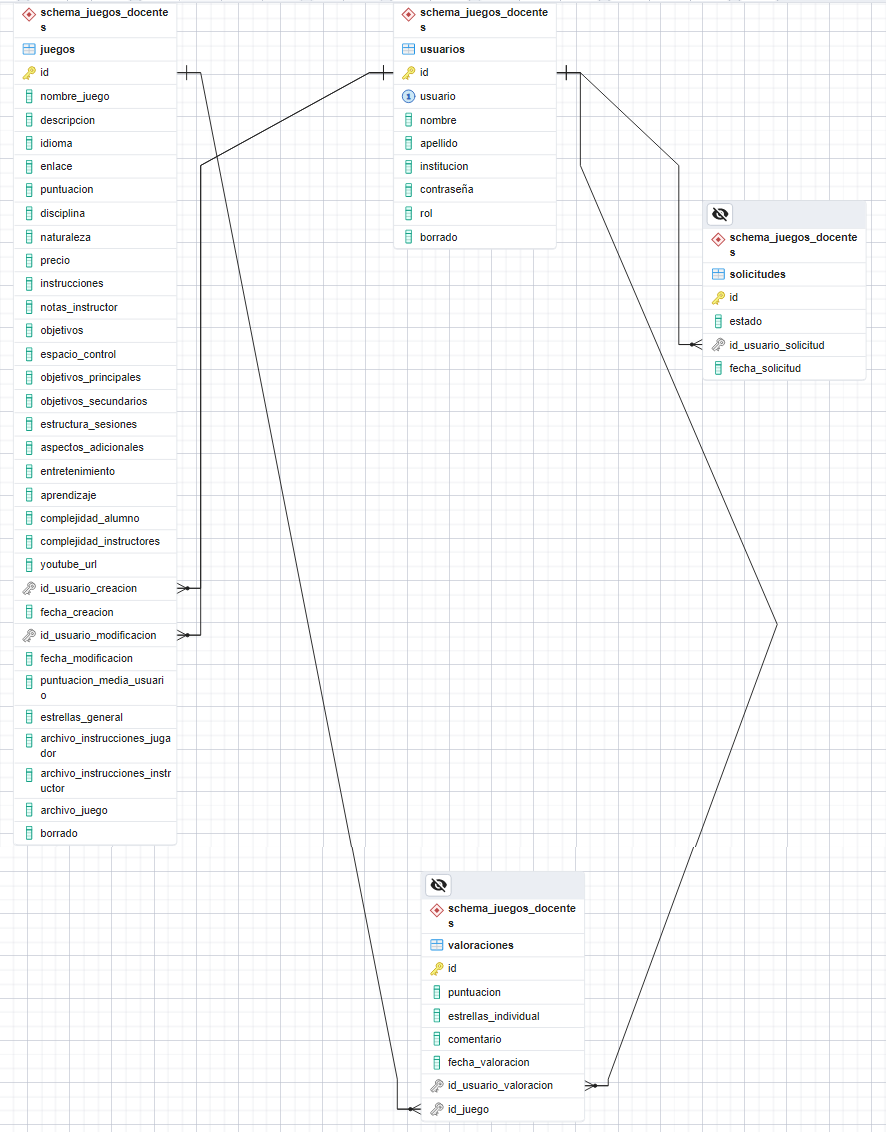
\includegraphics[width=1.0\textwidth]{ERD}
\caption{Modelo ERD.}
\label{fig:ERD}
\end{figure}

\newpage
\section{Diseño procedimental}
En esta sección se presentan los diagramas de secuencia de la aplicación, los cuales ilustran el funcionamiento y la interacción entre los diferentes componentes de la aplicación. 

\subsection{Registro}
Se muestra el diagrama de secuencia en la ejecución del registro.

\begin{figure}[!h]
\centering
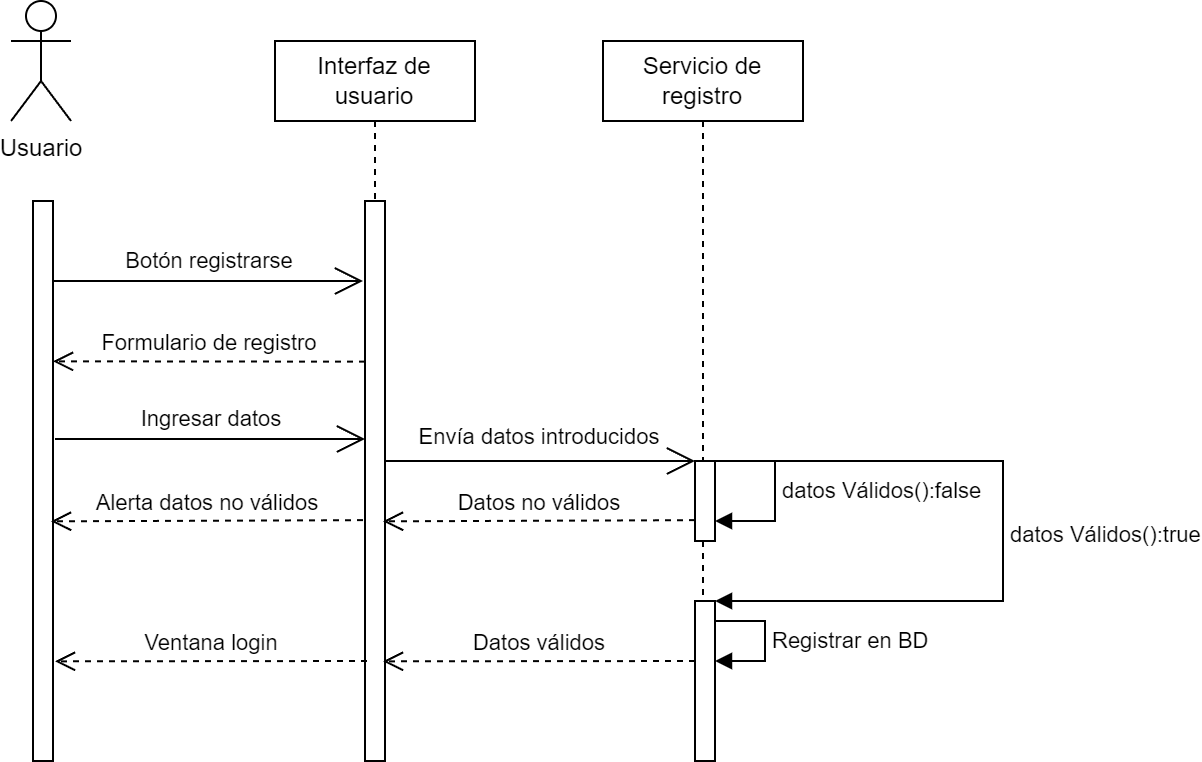
\includegraphics[width=1.0\textwidth]{diagrama-registro}
\caption{Diagrama de secuencia del registro.}
\label{fig:diagrama-secuencia-resgistro}
\end{figure}

\newpage
\subsection{Inicio sesión}
Se muestra el diagrama de secuencia en la ejecución del inicio de sesión.

\begin{figure}[!h]
\centering
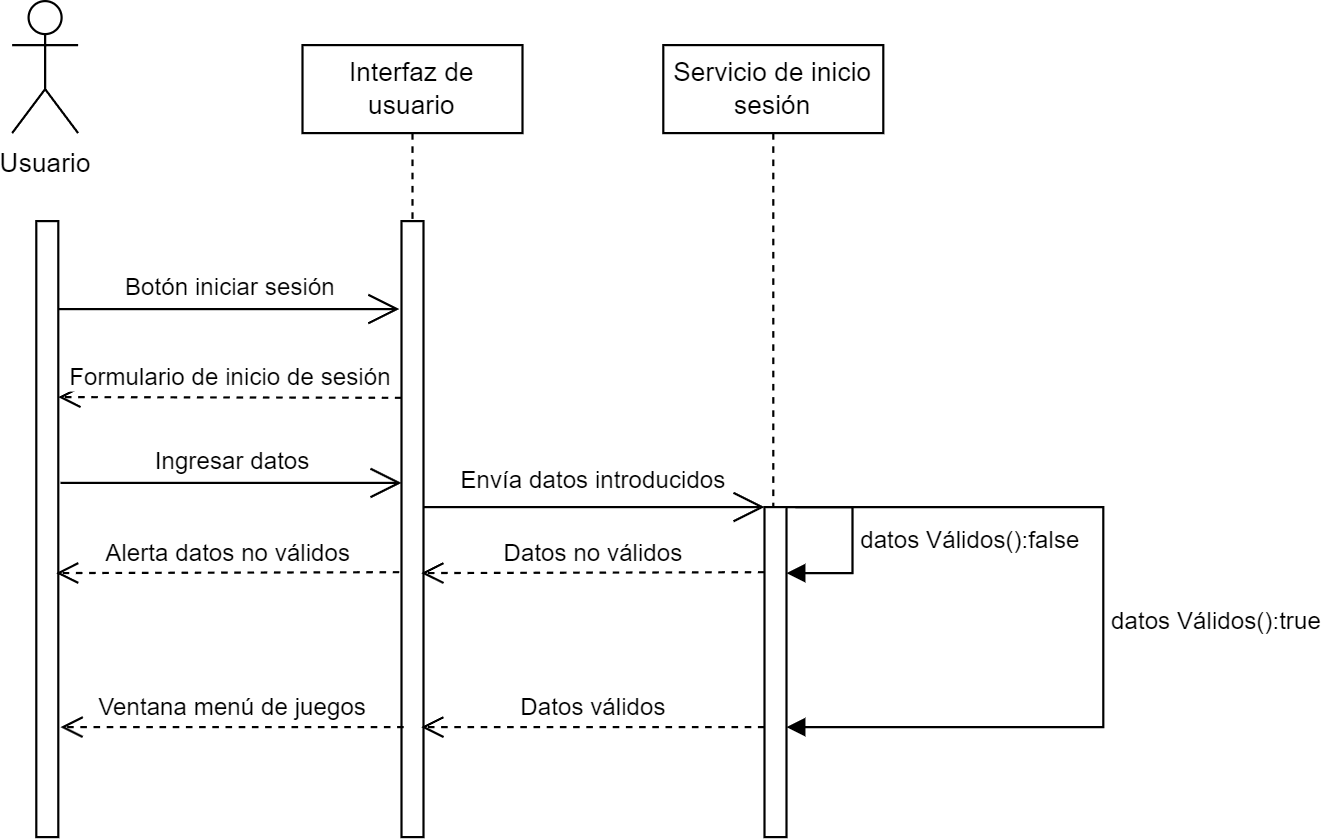
\includegraphics[width=1.0\textwidth]{diagrama-inicio}
\caption{Diagrama de secuencia del inicio de sesión.}
\label{fig:diagrama-secuencia-inicio-sesion}
\end{figure}

\newpage
\subsection{Visualización información de juego}
Se muestra el diagrama de secuencia en la ejecución de la visualización información de juego.
\begin{figure}[htb]
\centering
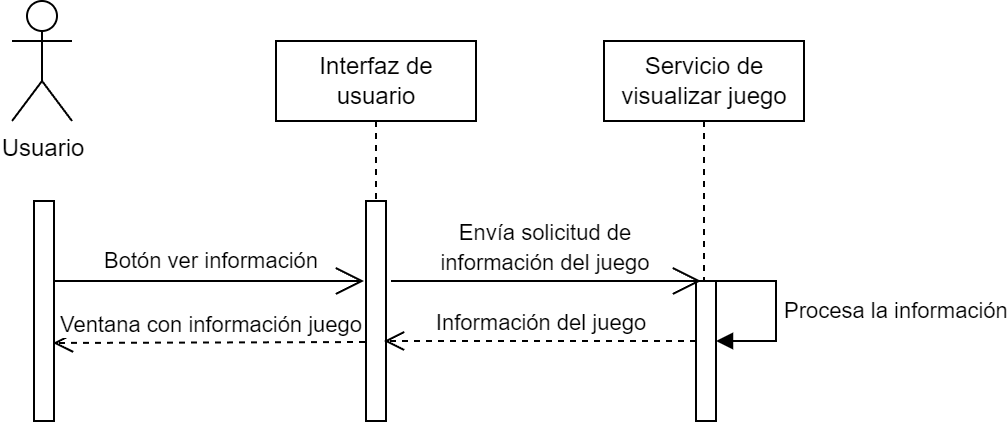
\includegraphics[width=0.9\textwidth]{diagrama-ver-juego}
\caption{Diagrama de secuencia del inicio de sesión.}
\label{fig:diagrama-secuencia-información-juego}
\end{figure}

\subsection{Visualización valoraciones de juego}
Se muestra el diagrama de secuencia en la ejecución de ver las valoraciones de un juego.
\begin{figure}[htb]
\centering
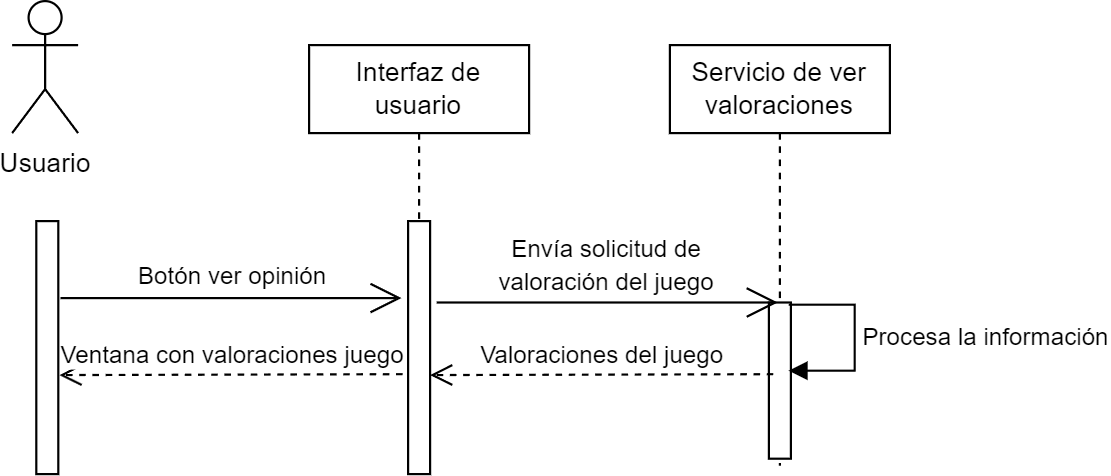
\includegraphics[width=1.0\textwidth]{diagrama-valoraciones}
\caption{Diagrama de secuencia de visualización de valoraciones.}
\label{fig:diagrama-secuencia-ver-valoraciones}
\end{figure}

\newpage
\subsection{Añadir valoración}
Se muestra el diagrama de secuencia en la ejecución de añadir una valoración a un juego.

\begin{figure}[htb]
\centering
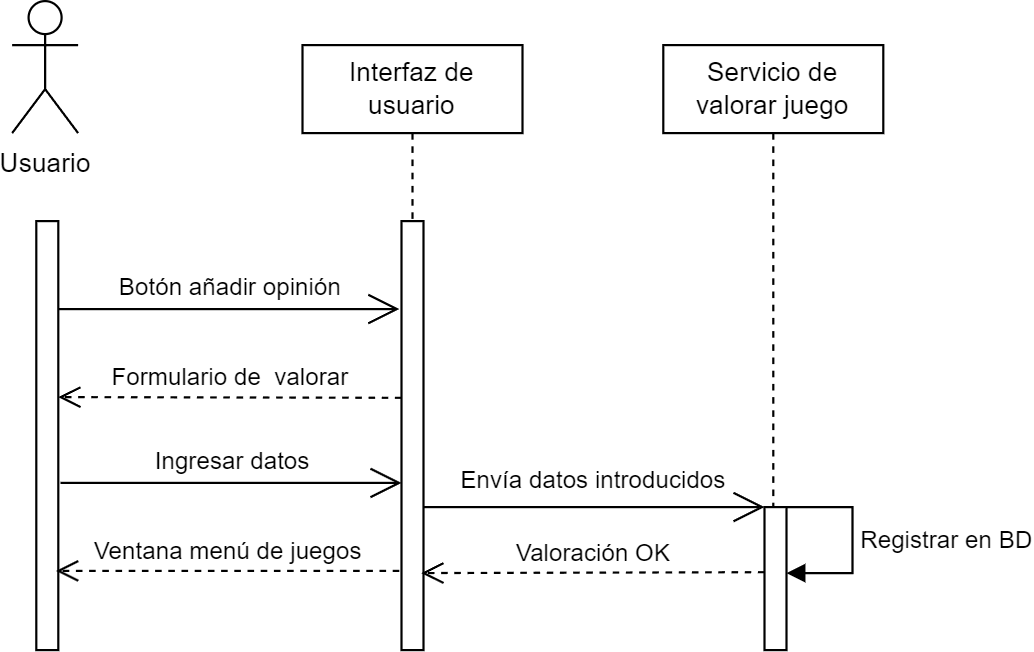
\includegraphics[width=1.0\textwidth]{diagrama-valorar-juego}
\caption{Diagrama de secuencia de añadir una valoración a un juego.}
\label{fig:diagrama-secuencia-añadir-valoración}
\end{figure}

\newpage
\subsection{Añadir juego}
Se muestra el diagrama de secuencia en la ejecución de añadir un nuevo juego.

\begin{figure}[h!]
\centering
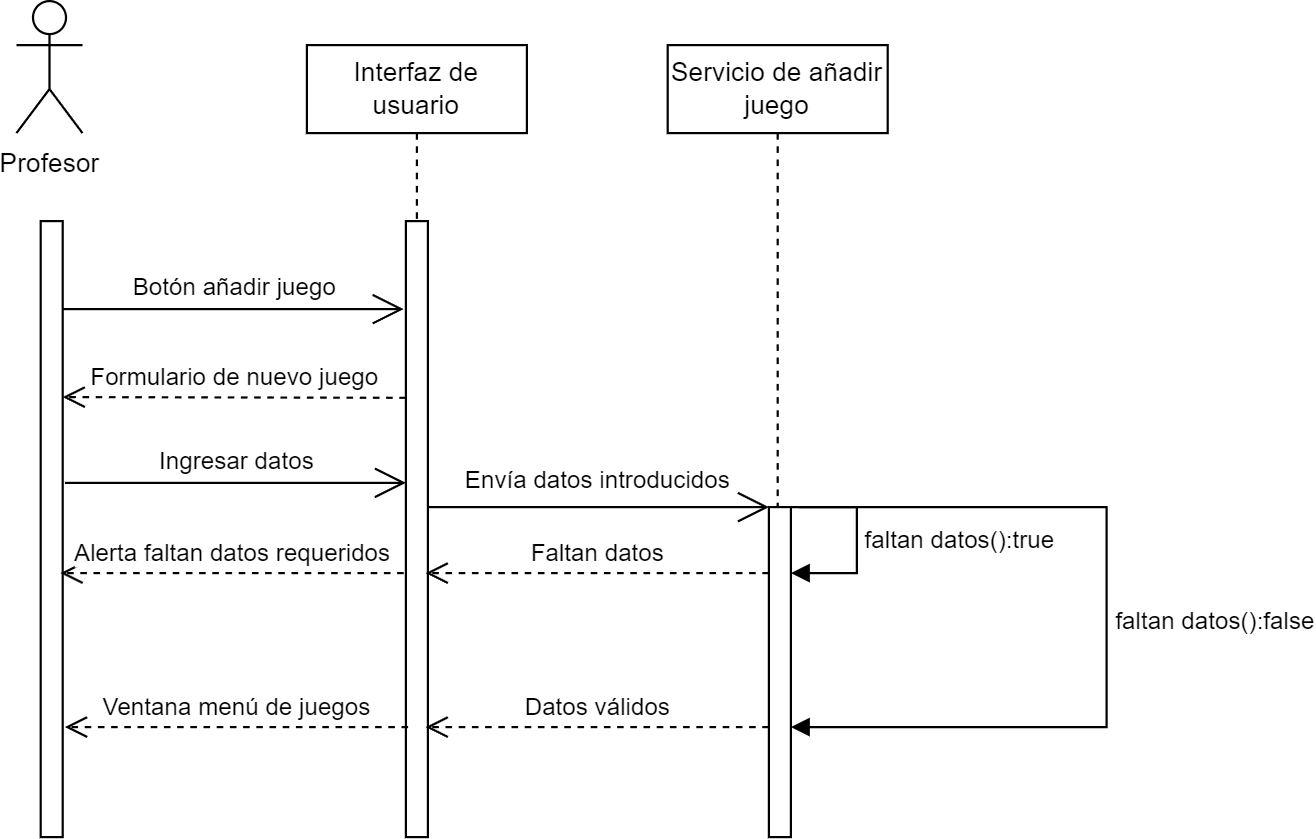
\includegraphics[width=1.0\textwidth]{diagrama-añadir-juego}
\caption{Diagrama de secuencia de añadir juego.}
\label{fig:diagrama-secuencia-añadir-juego}
\end{figure}

\newpage
\subsection{Modificar juego}
Se muestra el diagrama de secuencia en la ejecución de añadir un nuevo juego.

\begin{figure}[h!]
\centering
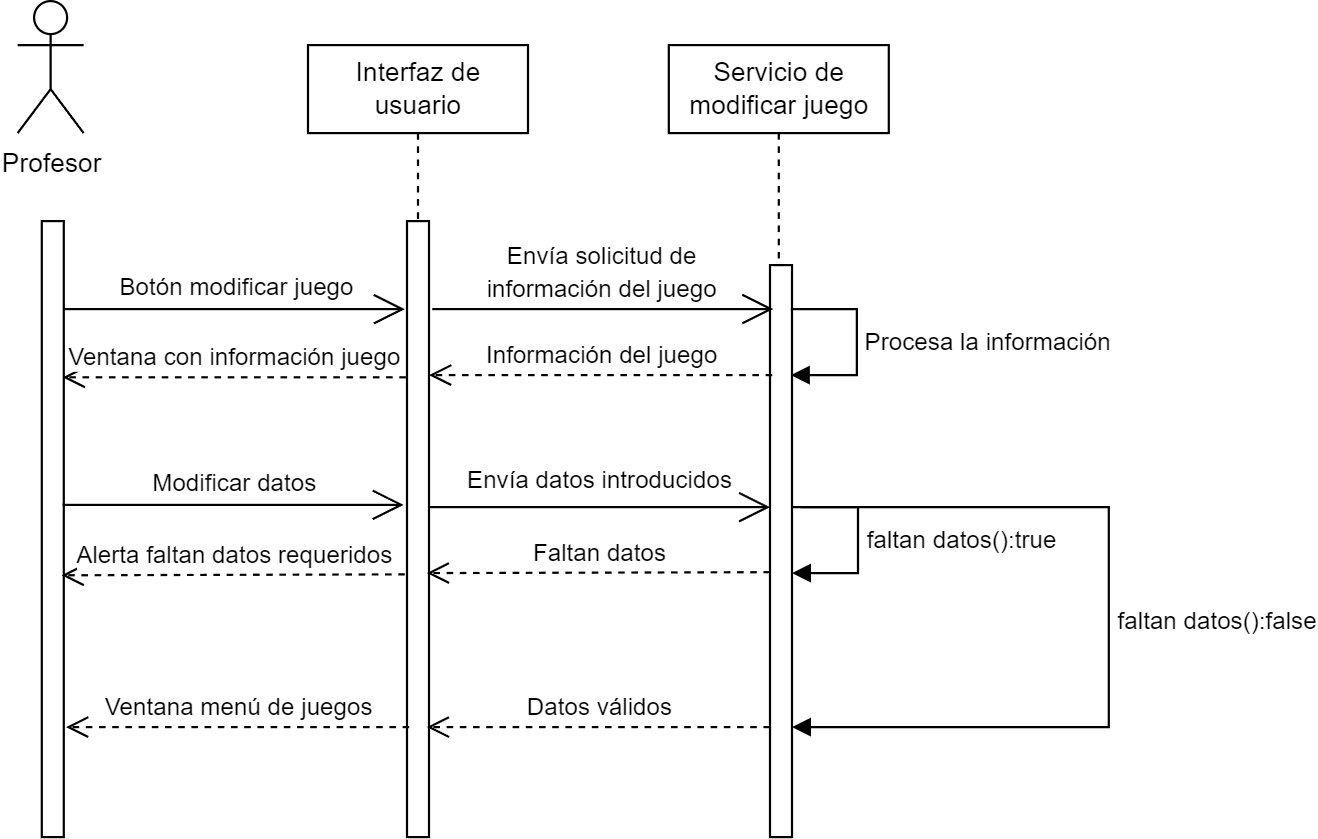
\includegraphics[width=1.0\textwidth]{diagrama-modificar-juego}
\caption{Diagrama de secuencia de modificar un juego.}
\label{fig:diagrama-secuencia-modificar-juego}
\end{figure}

\newpage
\subsection{Añadir archivos}
Se muestra el diagrama de secuencia en la ejecución de añadir archivos a la información del juego.

\begin{figure}[h!]
\centering
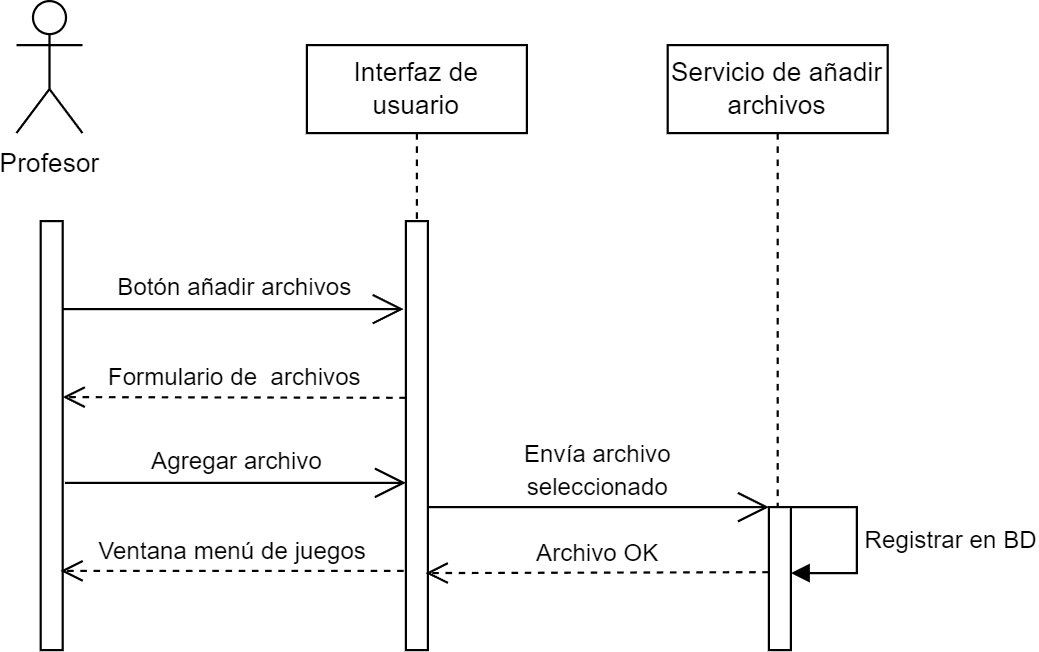
\includegraphics[width=1.0\textwidth]{diagrama-añadir-archivos}
\caption{Diagrama de secuencia de añadir archivos.}
\label{fig:diagrama-secuencia-añadir-archivos}
\end{figure}

\newpage
\subsection{Administración}
Se muestra el diagrama de secuencia en la ejecución de la administración.
\begin{figure}[h!]
\centering
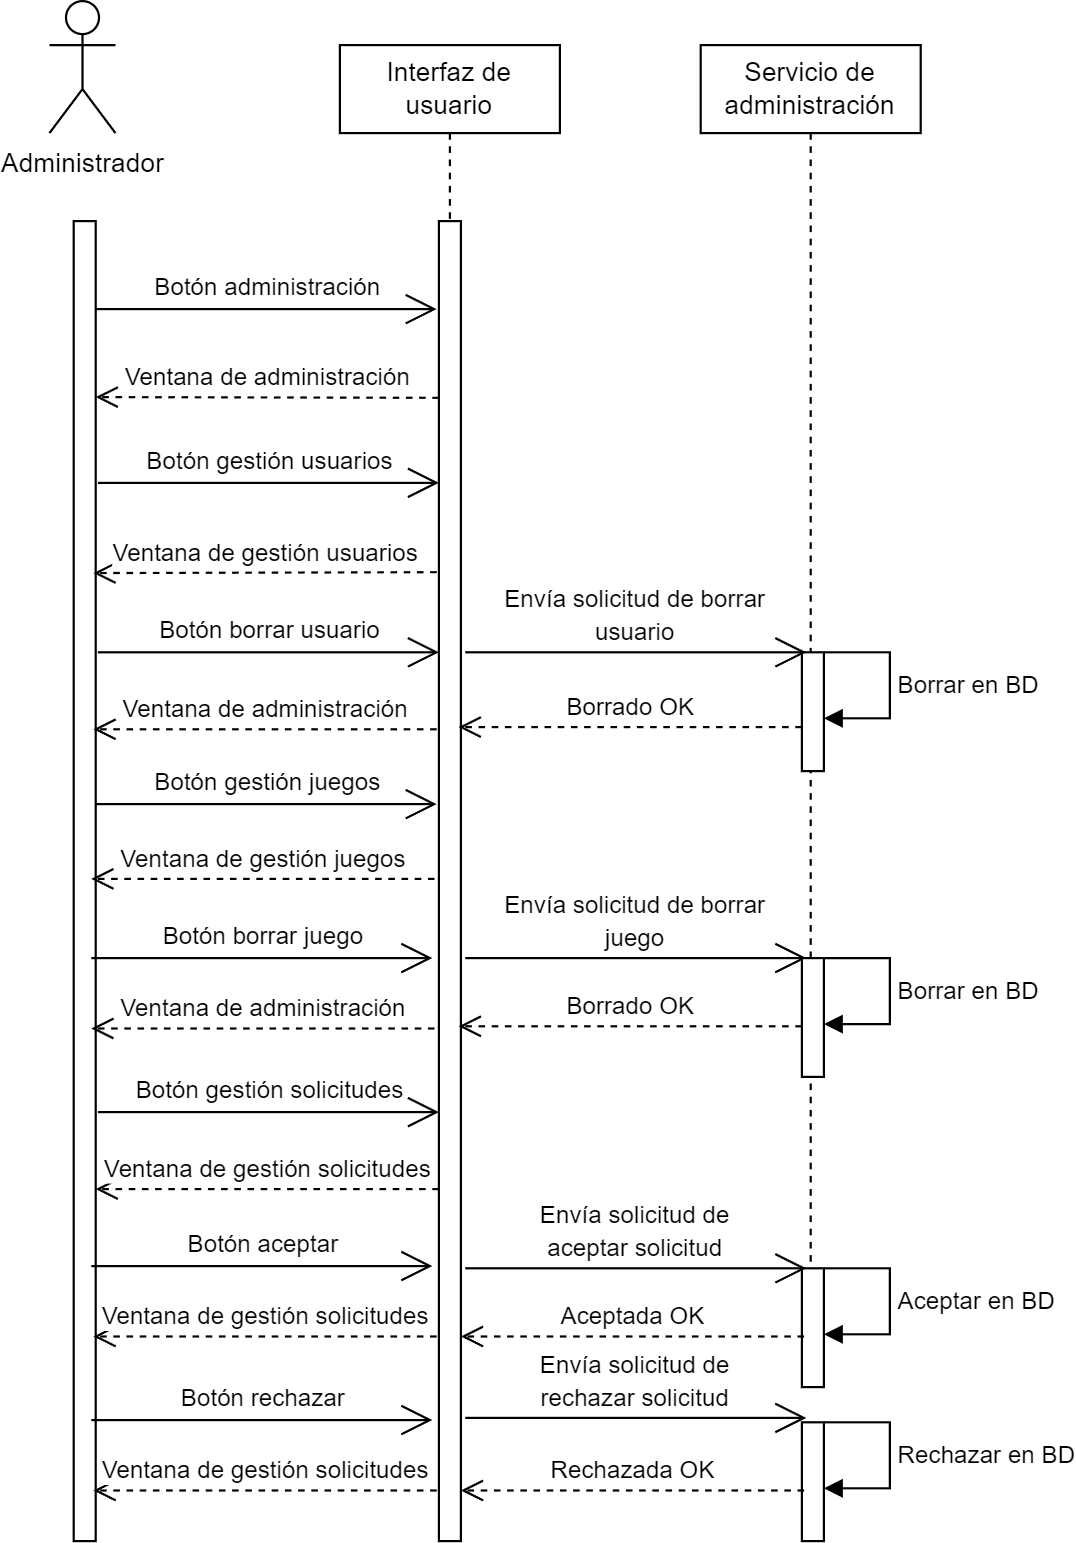
\includegraphics[width=0.8\textwidth]{diagrama-administracion}
\caption{Diagrama de secuencia de administración.}
\label{fig:diagrama-secuencia-administración}
\end{figure}

\newpage
\subsection{Modelo-Vista-Controlador (MVC)}
La arquitectura MVC, compuesta por el modelo, la vista y el controlador, separa los datos de la aplicación, la interfaz de usuario y la lógica de control.

En la aplicación, cada parte se atribuye de la siguiente manera:
\begin{itemize}
    \item\textbf{Modelo:} compuesto por los archivos database.py, juego.py, usuario.py, valoracion.py y solicitud.py. Estos archivos interactúan con la base de datos, realizando operaciones de creación, lectura, actualización y eliminación de los datos.
    \item\textbf{Vista:} compuesta por los templates HTML que presentan la visualización de las interfaces de usuario.
    \item\textbf{Controlador:} compuesto por el archivo app.py, ya que se encarga de la comunicación con los servicios de la vista. Maneja la interacción entre el modelo y la vista, devolviendo la información deseada.
\end{itemize}

\subsection{Fachada}
El patrón Fachada es un diseño estructural que proporciona una interfaz simplificada y unificada al cliente. Este patrón se emplea para simplificar la interacción del usuario con un subsistema más grande y complejo, como los módulos que se encargan de las operaciones en la base de datos en nuestra aplicación. En este sentido, el módulo app.py cumple el rol de fachada, ya que se encarga de comunicar los demás módulos con el cliente, proporcionando una interfaz coherente y simplificada.


\section{Diseño de interfaces}
Para la realización del proyecto se desarrolló el prototipo de las interfaces de la aplicación web mediante el uso de la herramienta de diseño Figma, con el fin de establecer inicialmente cómo iba a ser la aplicación web.

\subsection{Inicio}
La primera interfaz que se diseñó fue el prototipo de la página principal de inicio de la aplicación. Esta interfaz permite a los usuarios registrarse, iniciar sesión y comenzar a utilizar el repositorio de juegos, así como acceder a otras funcionalidades. Dependiendo del tipo de inicio de sesión (usuario, profesor o administrador), se les permitirá realizar diferentes acciones y acceder a diferentes funcionalidades.

\begin{figure}[htb]
\centering
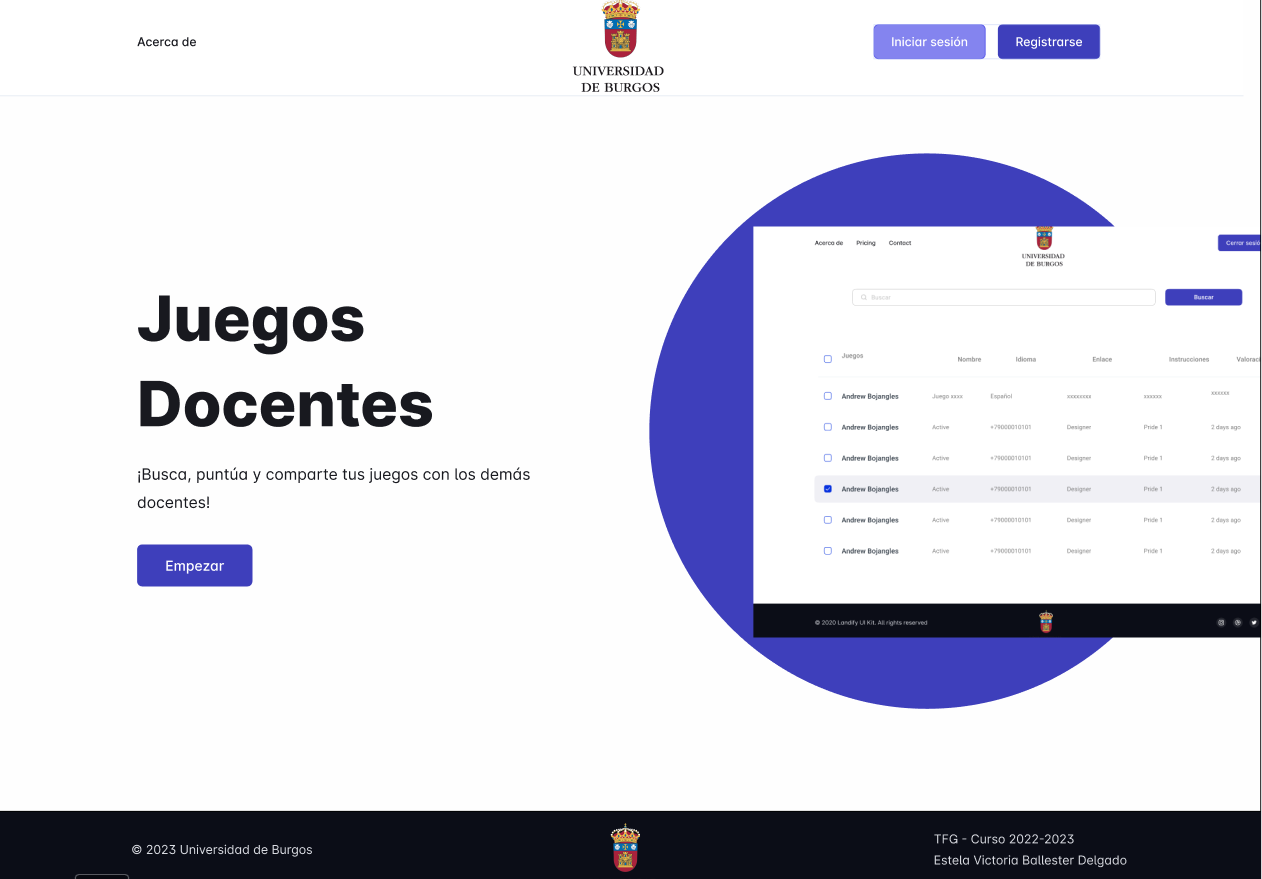
\includegraphics[width=0.7\textwidth]{inicio-prototipo}
\caption{Prototipo del inicio.}
\label{fig:inicio-prototipo}
\end{figure}

Finalmente, el resultado del template inicio.html quedó de la siguiente manera:

\begin{figure}[htb]
\centering
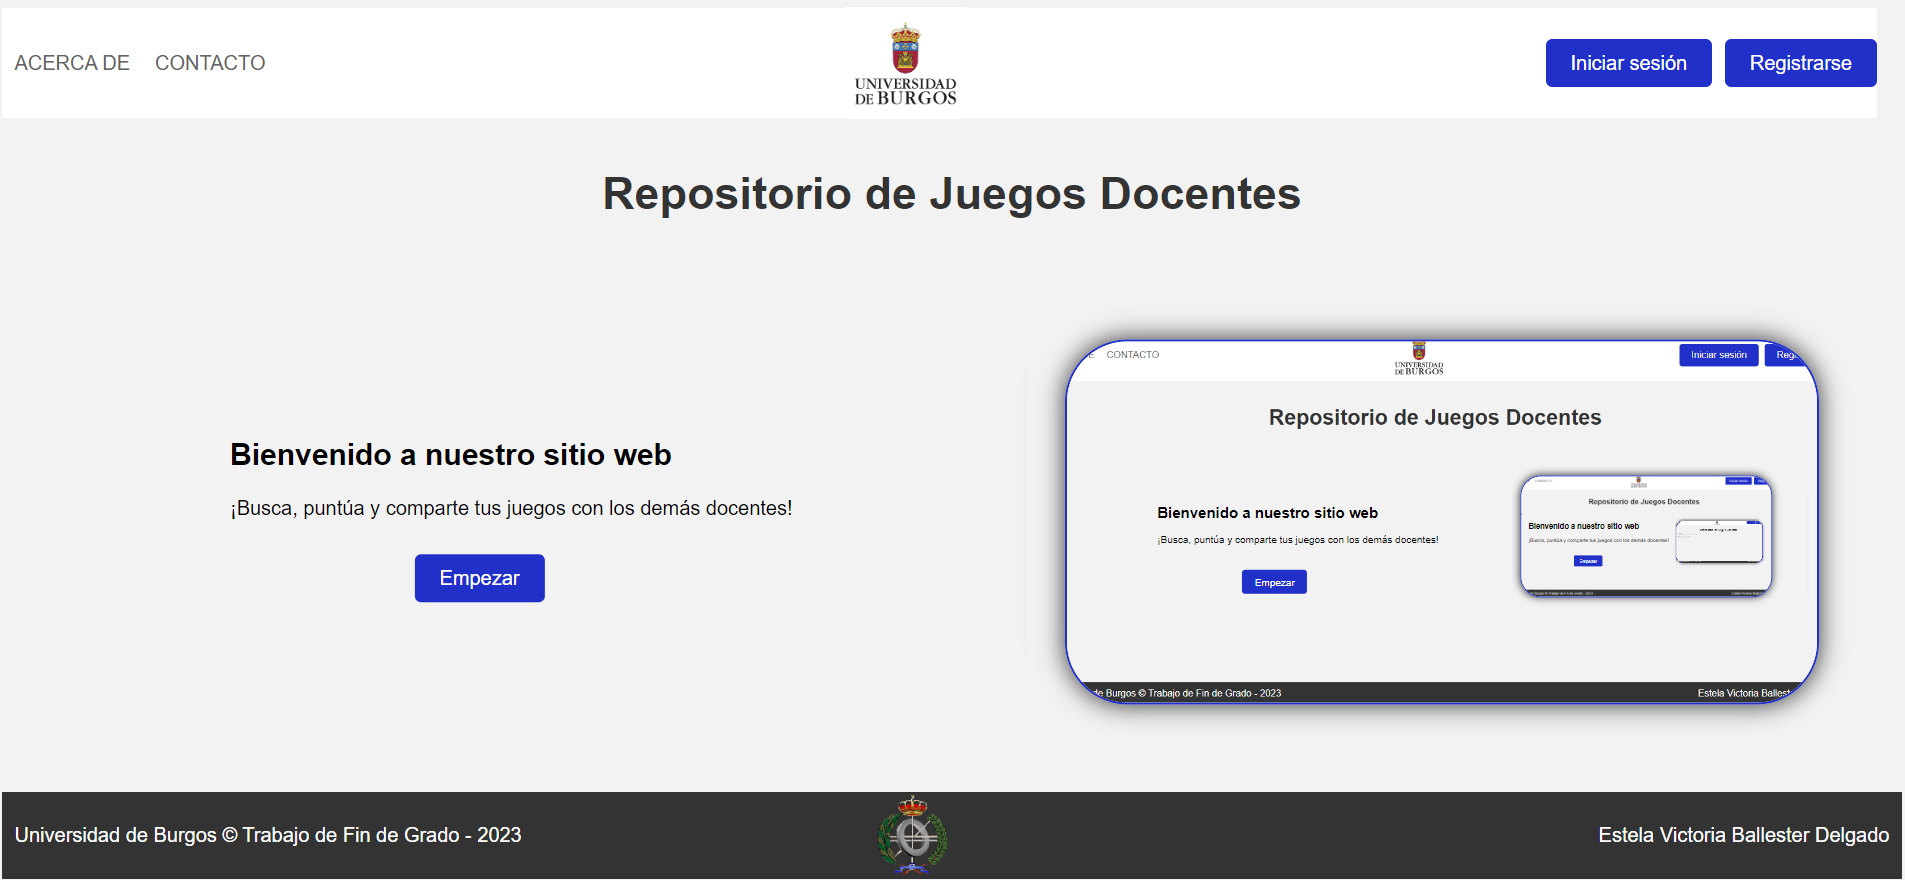
\includegraphics[width=0.8\textwidth]{inicio}
\caption{Interfaz del inicio.}
\label{fig:inicio}
\end{figure}

Como se puede apreciar, el resultado final del template inicio.html es prácticamente idéntico al prototipo en cuanto a funcionalidad. El diseño y la disposición de los elementos no se han mantenido tan fieles a la idea inicial, pero se refleja una buena implementación y una coherencia visual en la aplicación.

\subsection{Registro}
La interfaz de registro solicita al usuario introducir una serie de campos obligatorios entre los que se incluyen el nombre, la universidad y la contraseña. En el caso de tener ya una cuenta permite iniciar sesión desde ahí.

\begin{figure}[htb]
\centering
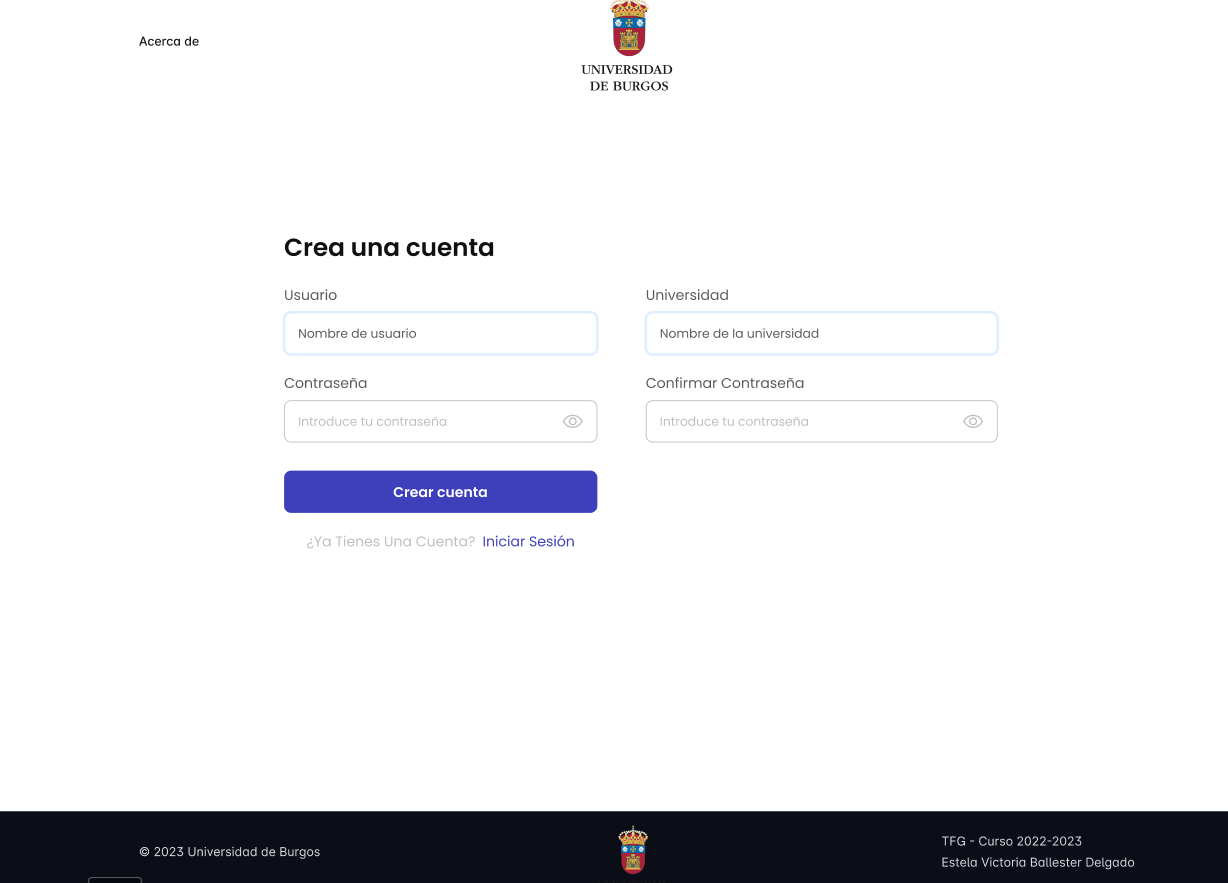
\includegraphics[width=0.7\textwidth]{registro-prototipo}
\caption{Prototipo del registro.}
\label{fig:registro-prototipo}
\end{figure}

Finalmente, el resultado del template registro.html quedó de la siguiente manera:

\begin{figure}[htb]
\centering
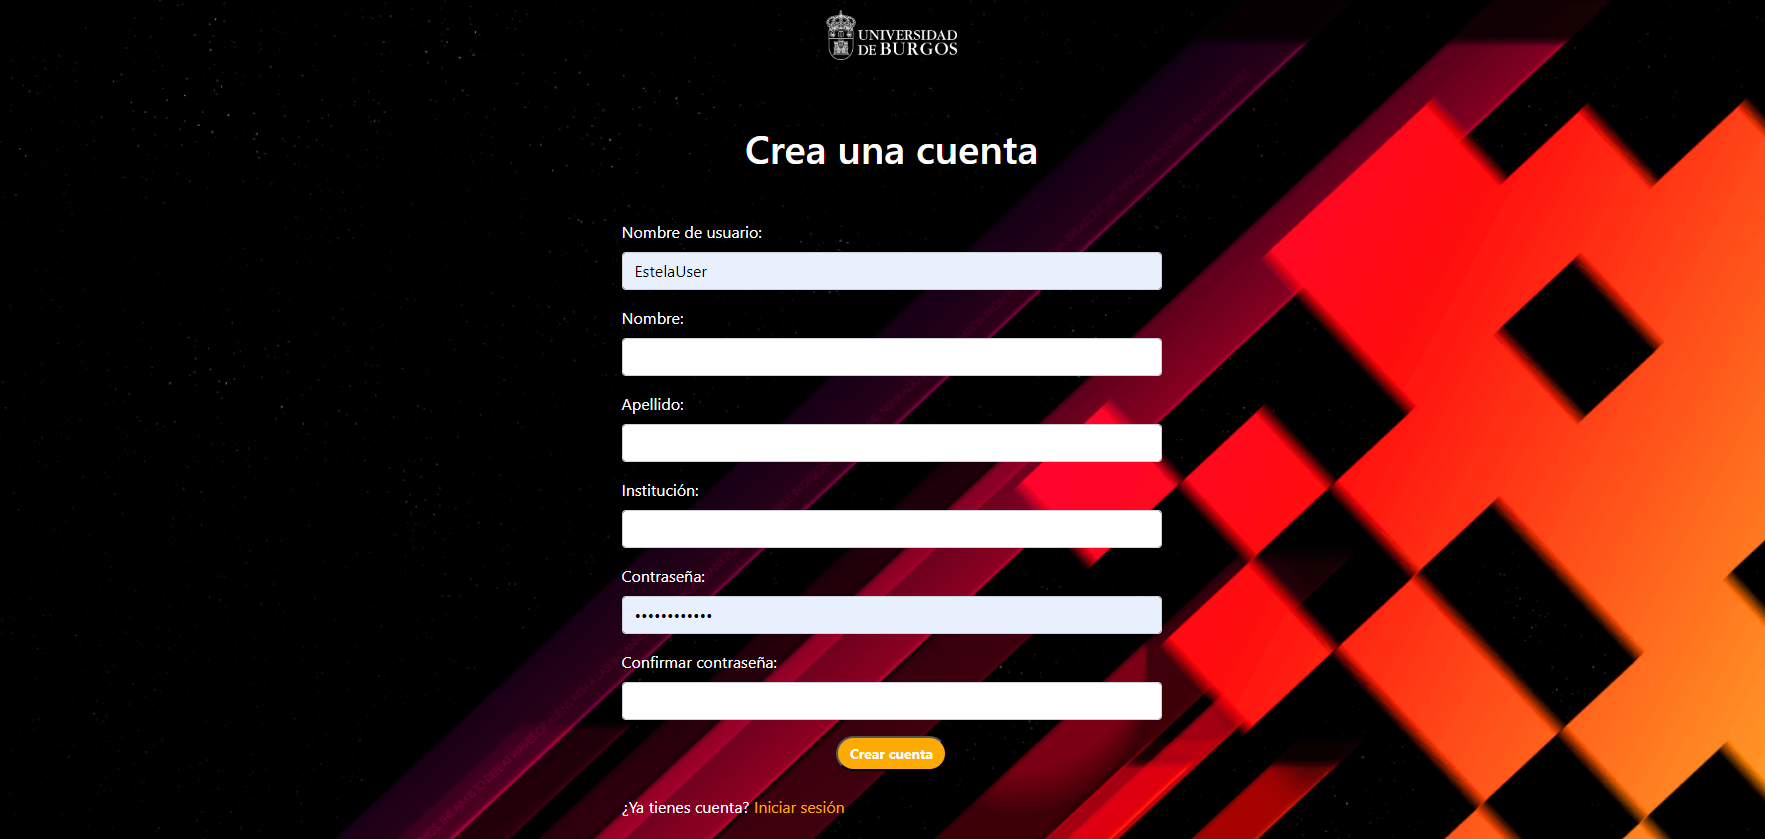
\includegraphics[width=0.8\textwidth]{registro}
\caption{Interfaz del registro.}
\label{fig:registro}
\end{figure}

Como se puede observar, el resultado final del template registro.html es prácticamente idéntico al prototipo inicial. Sin embargo, se han realizado algunas modificaciones para mejorar la funcionalidad del formulario de registro. En particular, se han agregado campos obligatorios adicionales, como el nombre y apellido del usuario, con el fin de recopilar información más completa durante el proceso de registro.

\subsection{Inicio de sesión}
La interfaz de inicio de sesión solicita al usuario introducir su nombre de usuario y la contraseña de su cuenta. También permite registrarse en el caso de no tener una cuenta creada. Además ofrece la posibilidad de recordar la contraseña si el usuario no la recuerda.

\begin{figure}[htb]
\centering
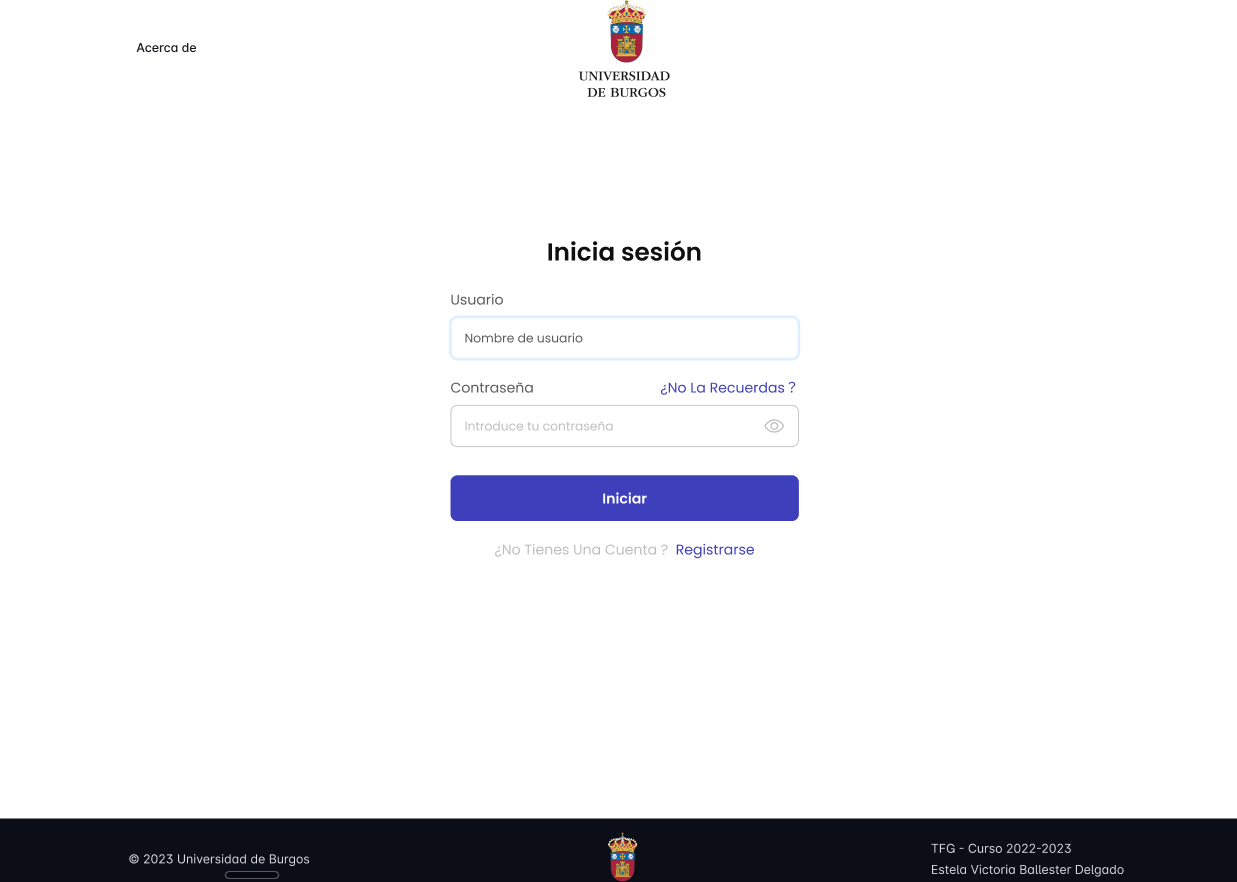
\includegraphics[width=0.7\textwidth]{login-prototipo}
\caption{Prototipo del inicio de sesión.}
\label{fig:login-prototipo}
\end{figure}

Finalmente, el resultado del template login.html quedó de la siguiente manera:
\newpage
\begin{figure}[htb]
\centering
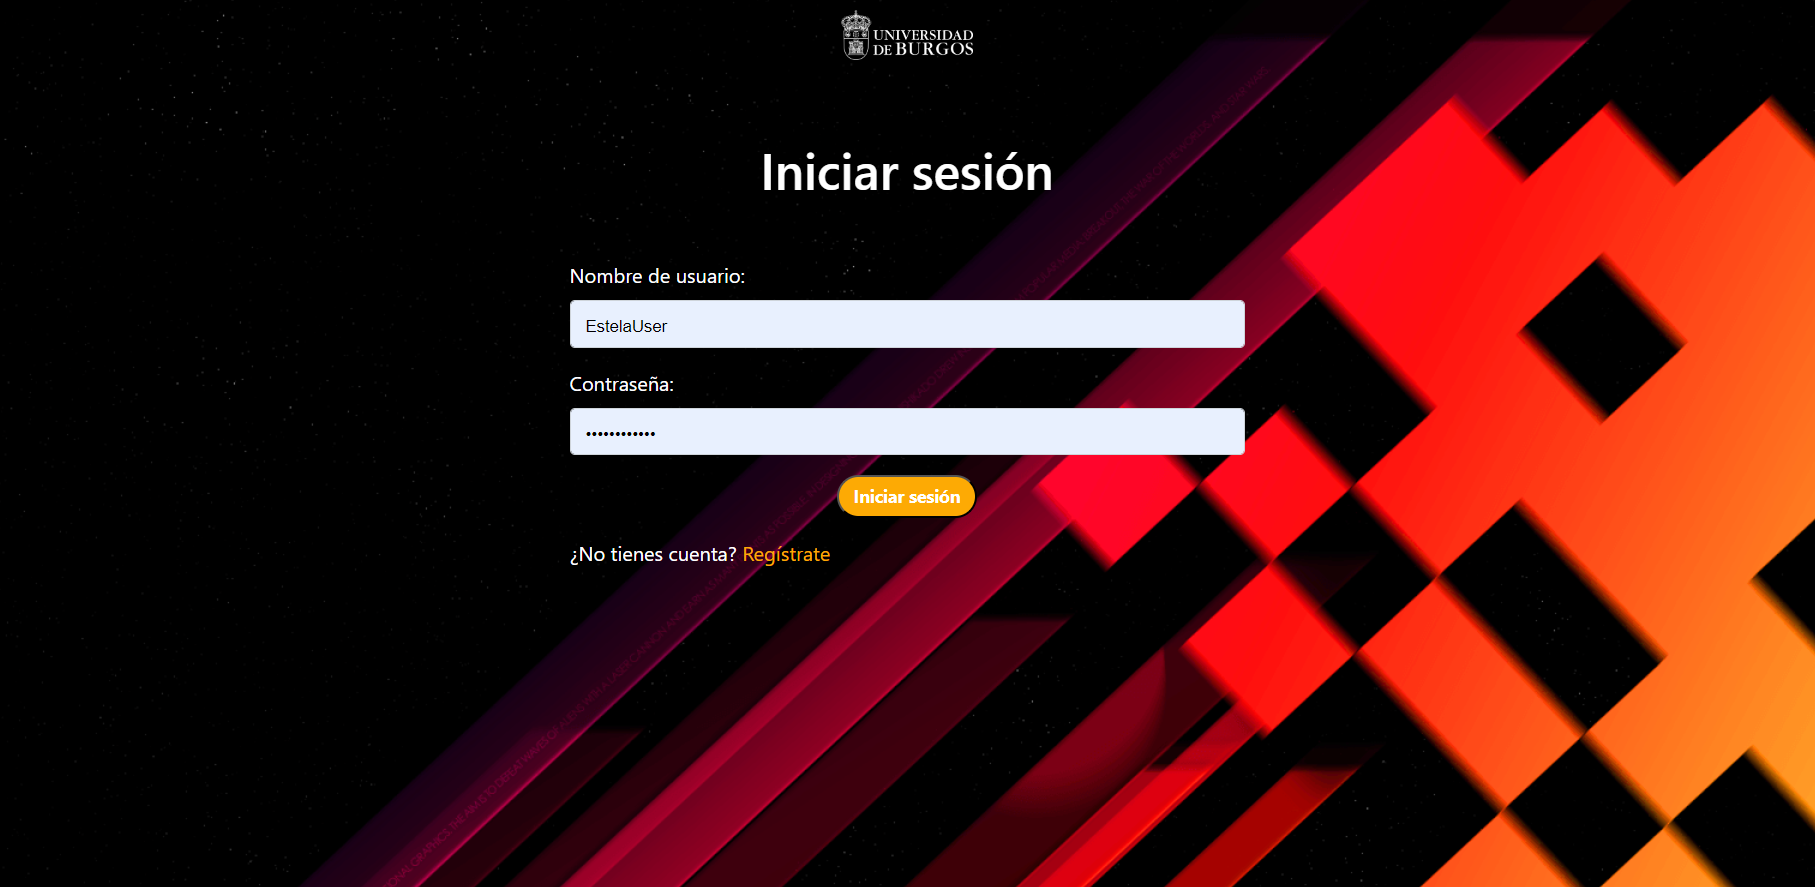
\includegraphics[width=0.8\textwidth]{login}
\caption{Interfaz del inicio de sesión.}
\label{fig:login}
\end{figure}

Como se puede observar, el resultado final del template login.html es prácticamente idéntico al prototipo inicial. Sin embargo, se diferencia en que finalmente no se implementó la funcionalidad de recuperación de contraseña en caso de olvido. Esta decisión se tomó con el objetivo de simplificar el proceso de inicio de sesión y priorizar otras funcionalidades importantes

\subsection{Menú de juegos de usuarios}
La interfaz del menú de juegos de los usuarios permite realizar búsquedas personalizadas de los juegos, visualizar la información detallada de cada juego y además brinda la opción de valorarlos.

\begin{figure}[htb]
\centering
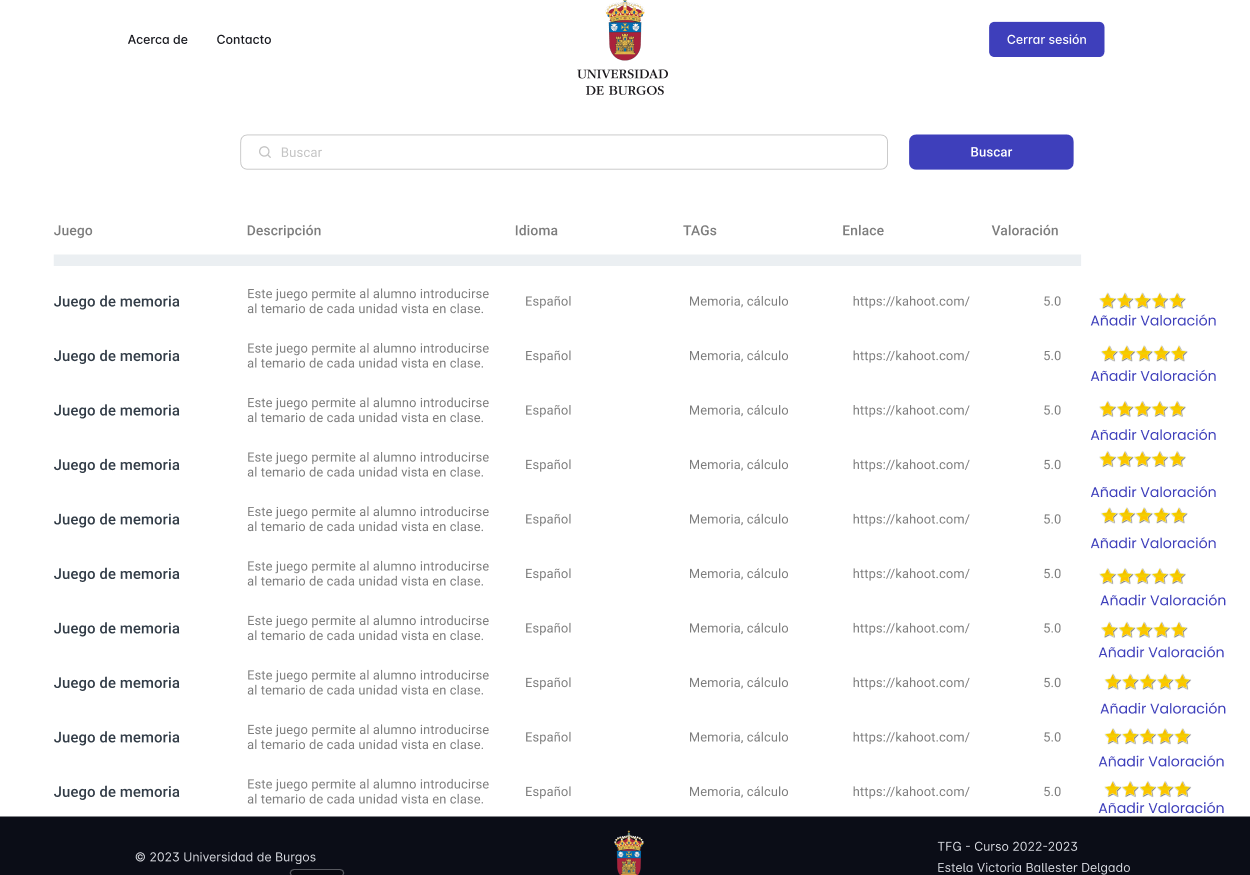
\includegraphics[width=0.7\textwidth]{menu-usuarios-prototipo}
\caption{Prototipo del menú de juegos de usuarios.}
\label{fig:menu-usuarios-prototipo}
\end{figure}

\newpage
Finalmente, el resultado del template menu\_juegos\_usuario.html quedó de la siguiente manera:

\begin{figure}[htb]
\centering
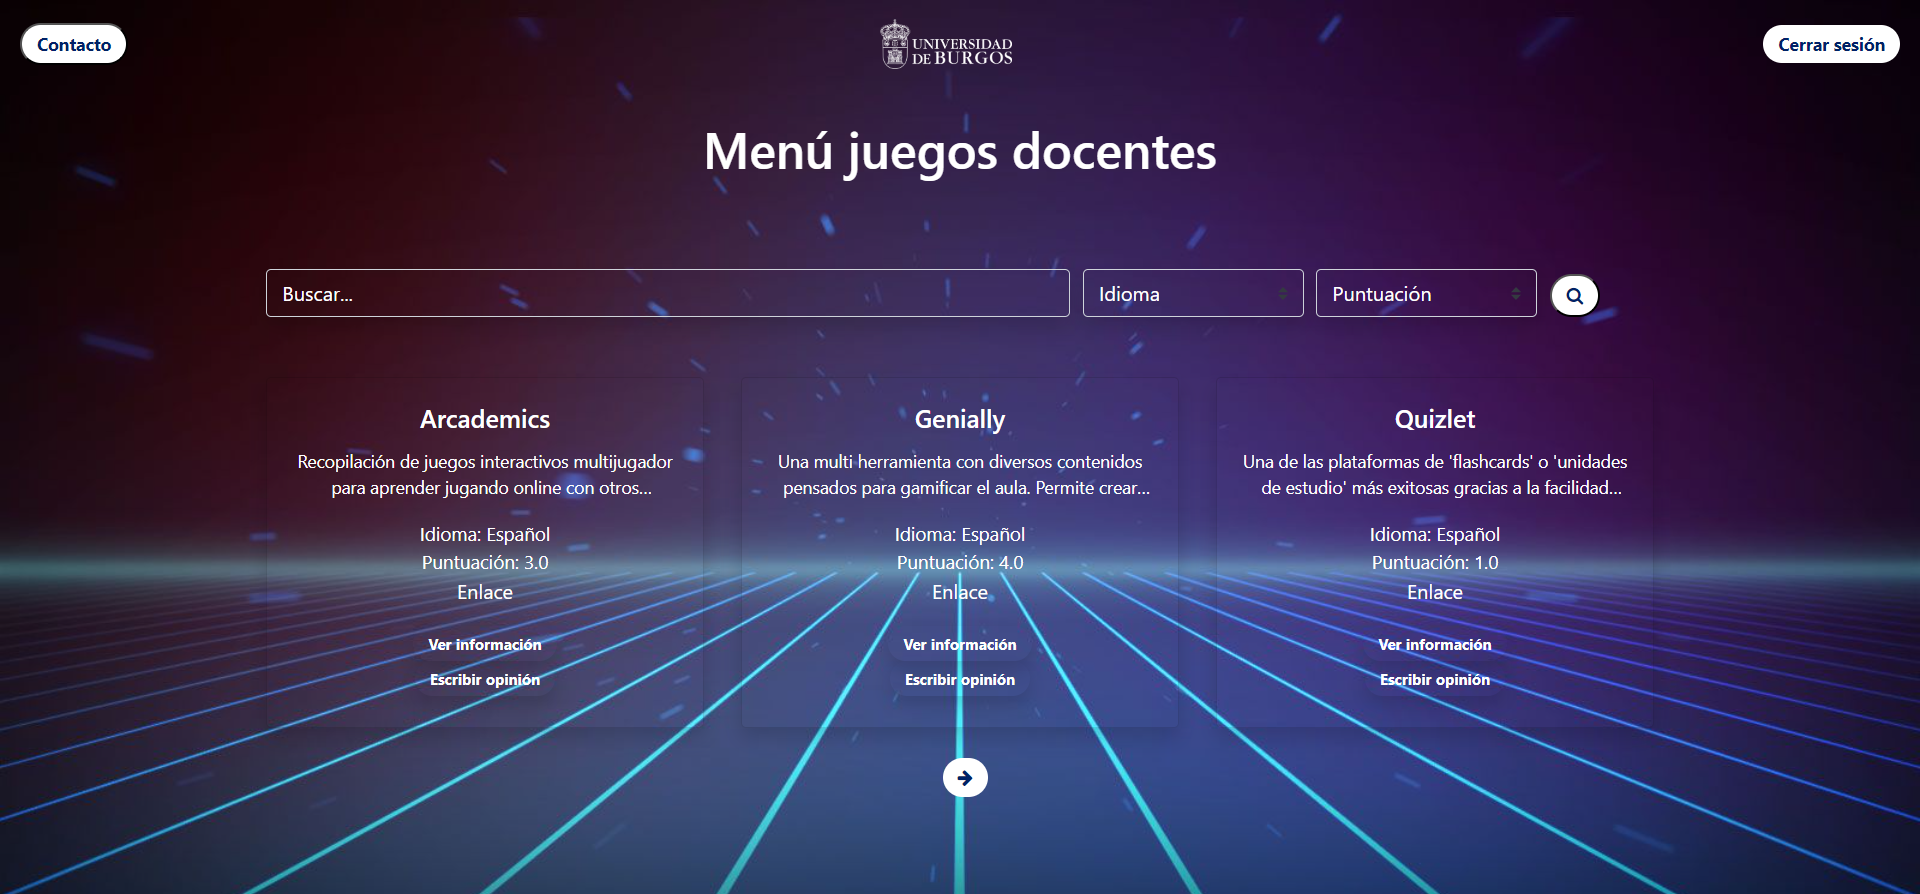
\includegraphics[width=0.7\textwidth]{menu-usuarios}
\caption{Interfaz del menú de juegos de usuarios.}
\label{fig:menu-usuarios}
\end{figure}

Como se puede observar, el resultado final del template menu\_juegos\_usuario.html presenta varias diferencias visuales en comparación con el prototipo inicial. La principal diferencia radica en la forma en que se muestran los juegos, ya que en el prototipo se mostraban en forma de tabla y en el resultado final se presentan en tarjetas, lo cual facilita su visualización. Además, en el resultado final se ha agregado la funcionalidad de realizar búsquedas utilizando tanto la barra de búsqueda como filtros, lo cual permite realizar búsquedas más específicas.

\subsection{Añadir valoración}
La interfaz de añadir una valoración a un juego permite introducir una puntuación y añadir un comentario escrito.

\begin{figure}[htb]
\centering
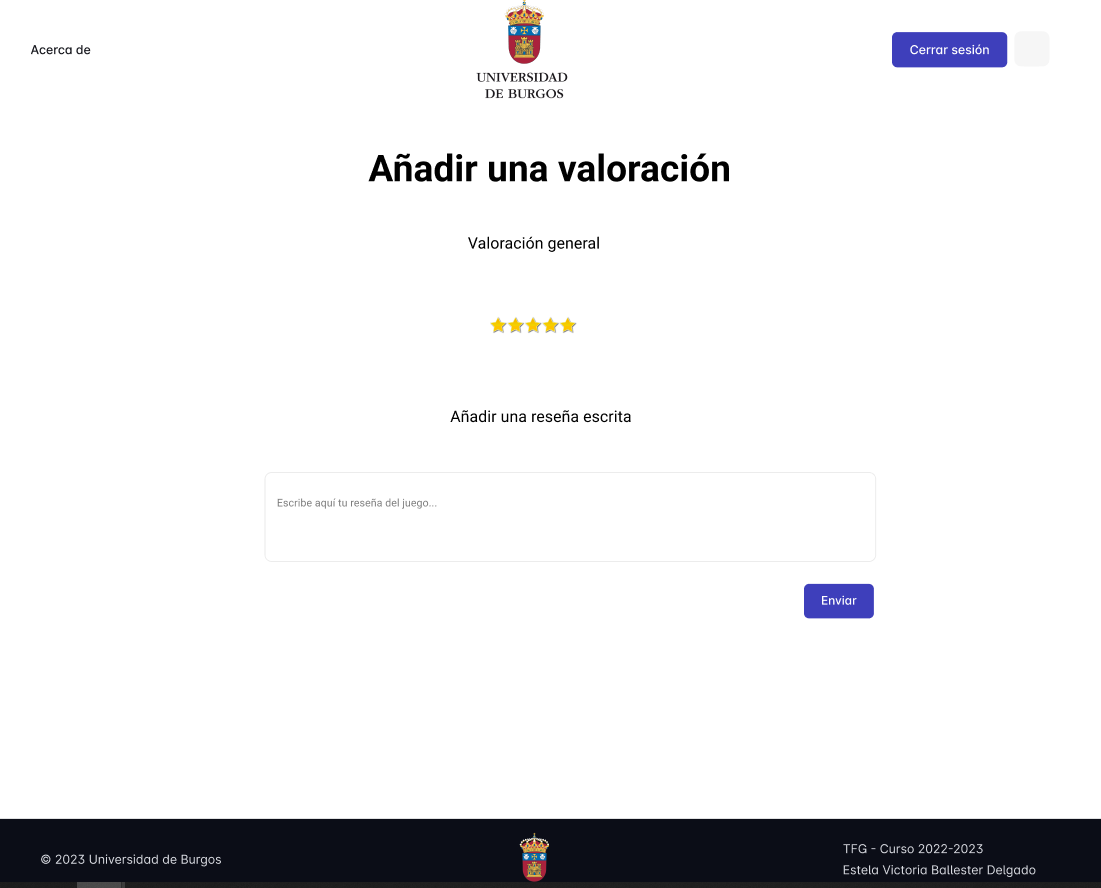
\includegraphics[width=0.7\textwidth]{añadir-valoracion-prototipo}
\caption{Prototipo de añadir una valoración.}
\label{fig:añadir-valoracion-prototipo}
\end{figure}

Finalmente, el resultado del template añadir\_valoracion.html quedó de la siguiente manera:

\begin{figure}[htb]
\centering
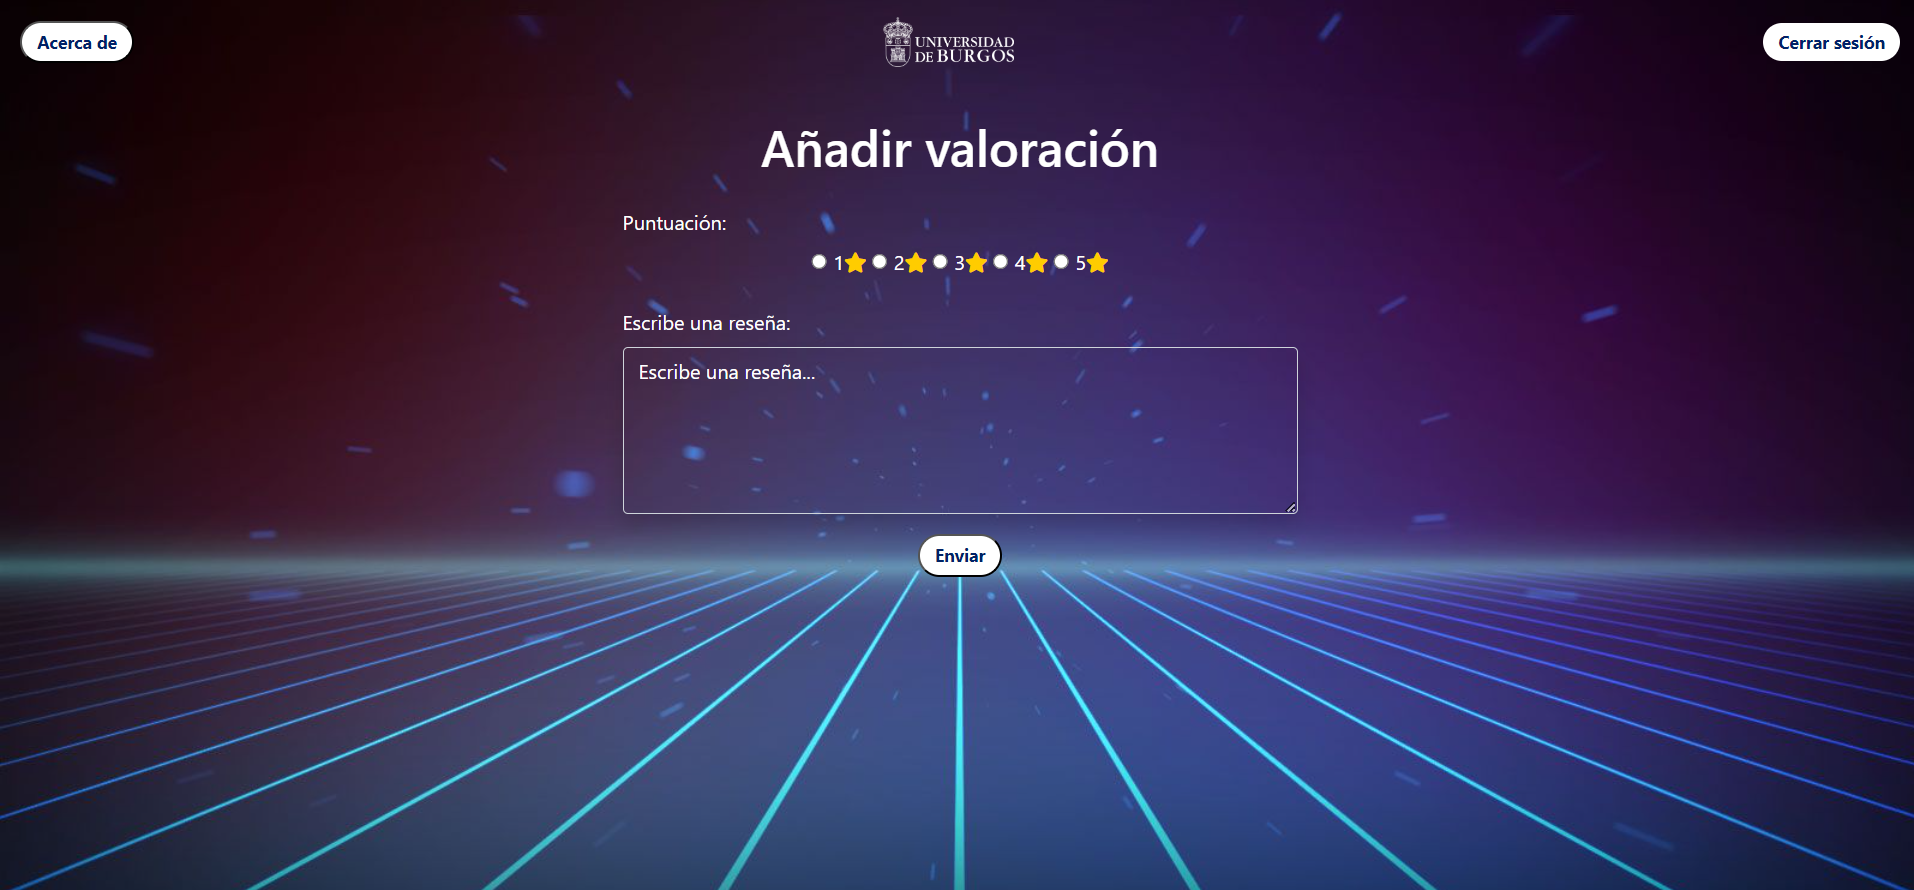
\includegraphics[width=0.8\textwidth]{añadir-valoracion}
\caption{Interfaz de añadir una valoración.}
\label{fig:añadir-valoracion}
\end{figure}

Como se puede observar, el resultado final del template añadir\_valoracion.html es prácticamente idéntico al prototipo inicial.

\subsection{Visualizar valoración}
La interfaz de visualizar las valoraciones de un juego permite ver todas las reseñas que han dejado los usuarios sobre dicho juego.

\begin{figure}[htb]
\centering
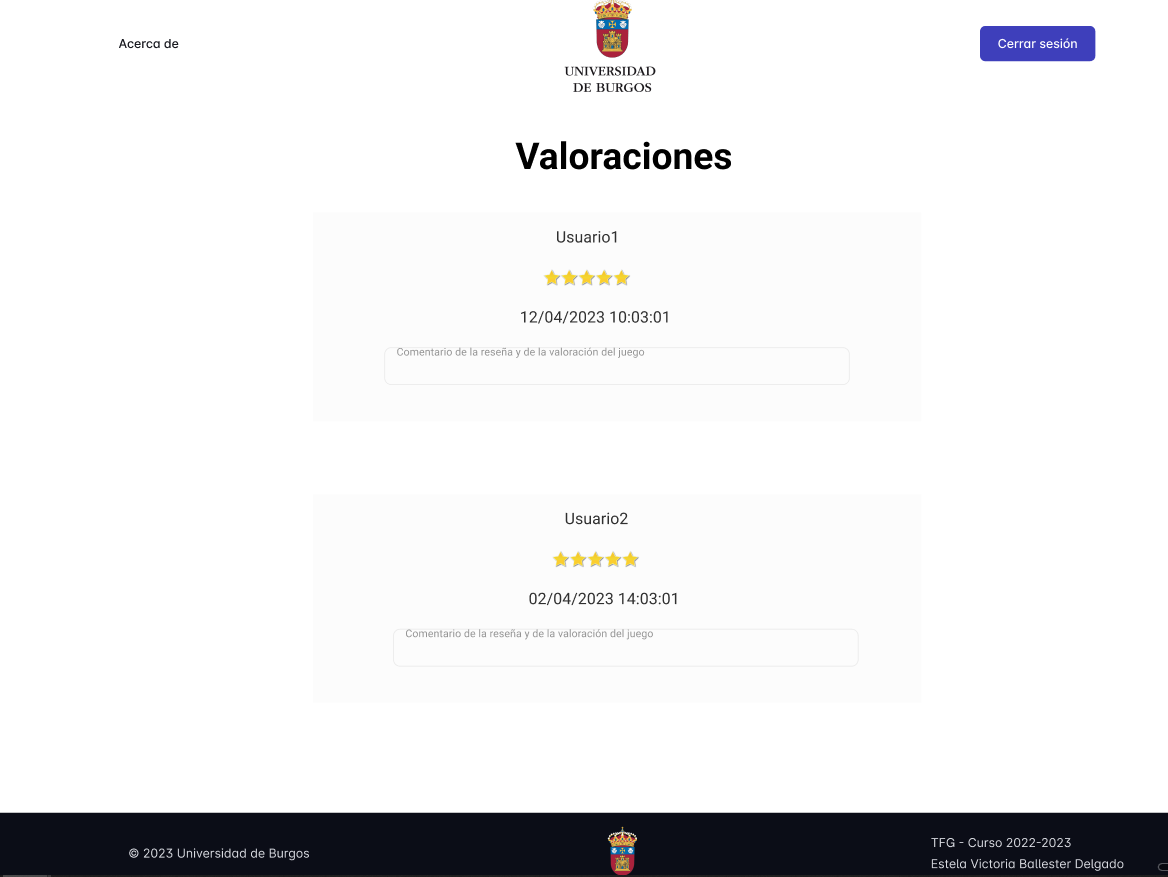
\includegraphics[width=0.7\textwidth]{visualizar-valoracion-prototipo}
\caption{Prototipo de la visualización de valoraciones.}
\label{fig:visualizar-valoracion-prototipo}
\end{figure}

Finalmente, el resultado del template visualizar\_valoracion.html quedó de la siguiente manera:

\begin{figure}[htb]
\centering
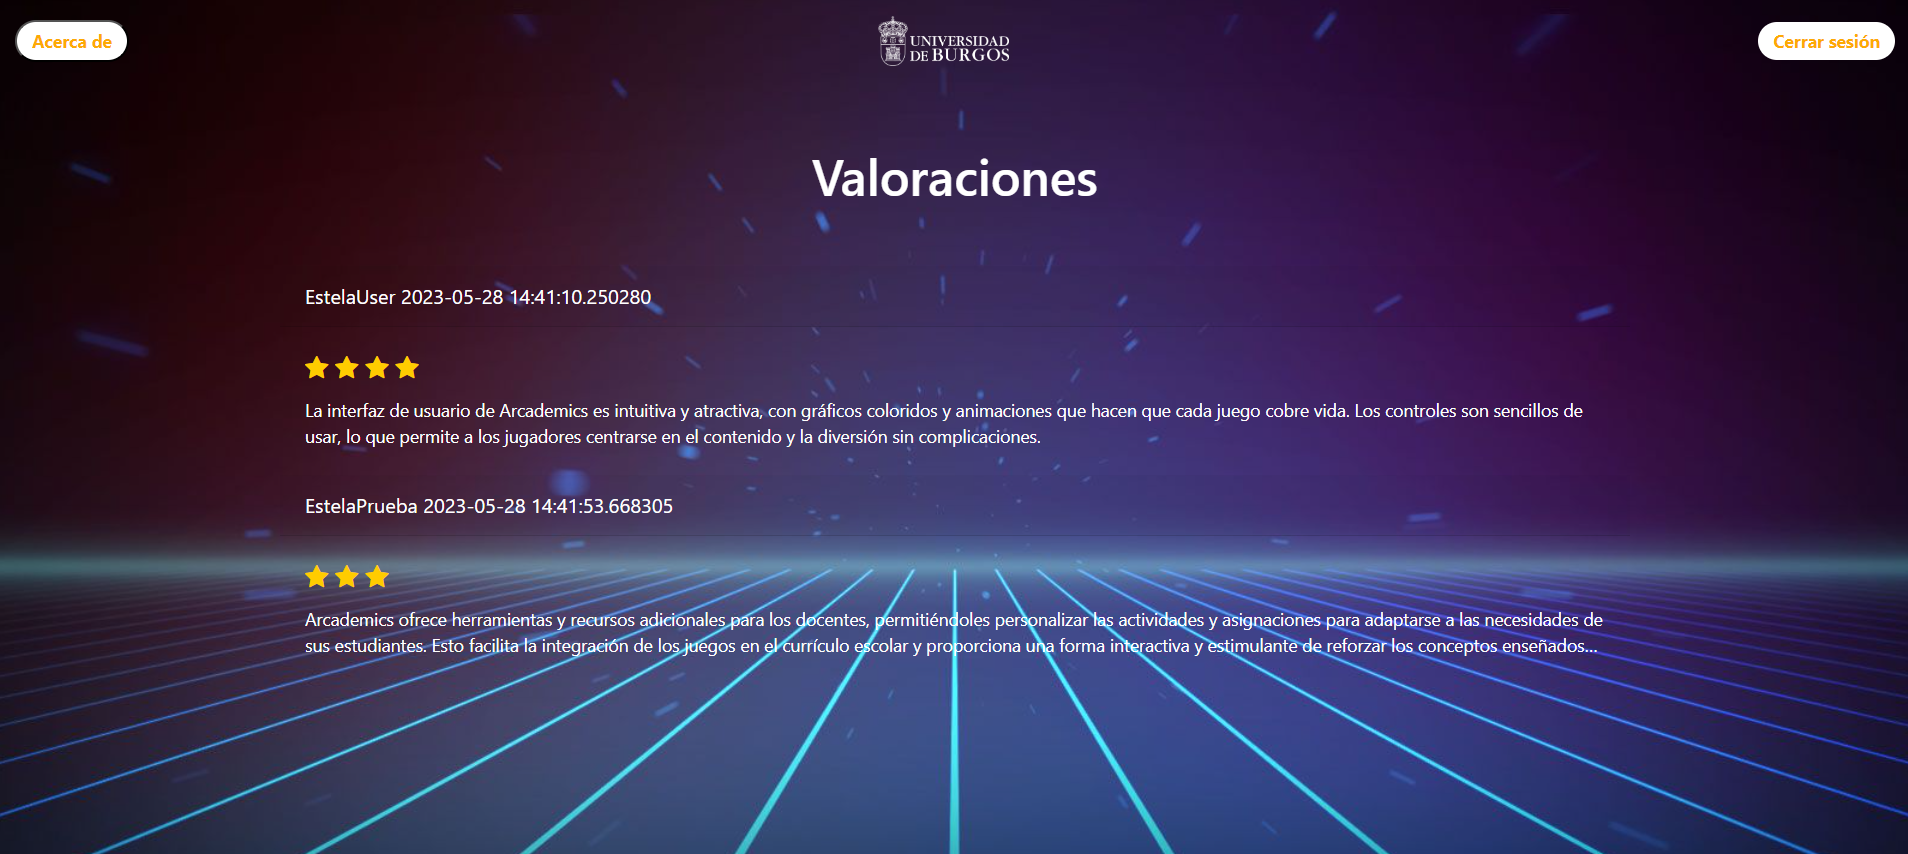
\includegraphics[width=0.8\textwidth]{visualizar-valoracion}
\caption{Interfaz de la visualización de valoraciones.}
\label{fig:visualizar-valoracion}
\end{figure}

Como se puede observar, el resultado final del template visualizar\_valoracion.html es prácticamente idéntico al prototipo inicial.

\subsection{Contacto}
La interfaz de contacto solo es accesible por los usuarios. Esta les permite solicitar el rol de profesor.

\begin{figure}[htb]
\centering

\includegraphics[width=0.7\textwidth]{solicitar}
\caption{Prototipo del contacto.}
\label{fig:solicitar}
\end{figure}

Finalmente, el resultado del template contacto.html quedó de la siguiente manera:

\begin{figure}[htb]
\centering

\includegraphics[width=0.8\textwidth]{contacto}
\caption{Interfaz del contacto.}
\label{fig:contacto}
\end{figure}

Como se puede observar, el resultado final del template contacto.html es prácticamente idéntico al prototipo inicial. 

\subsection{Menú de juegos de profesores}
La interfaz del menú de juegos de los profesores proporciona diversas funcionalidades. Permite realizar búsquedas personalizadas de los juegos, visualizar información detallada de cada juego, así como añadir nuevos juegos y modificar los existentes.

\begin{figure}[htb]
\centering
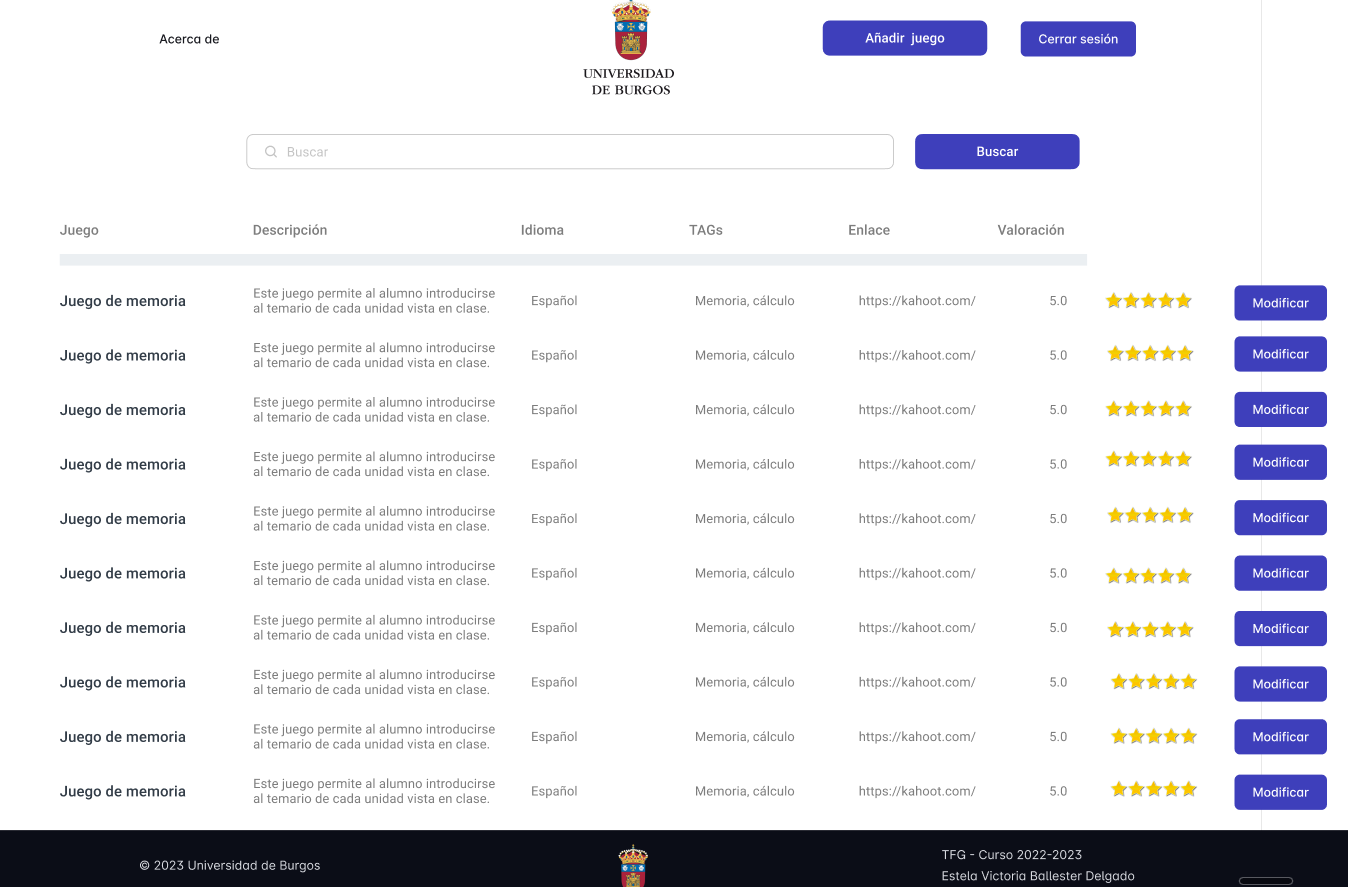
\includegraphics[width=0.7\textwidth]{menu-profesor-prototipo}
\caption{Prototipo del menú de juegos de profesores.}
\label{fig:menu-profesor-prototipo}
\end{figure}

Finalmente, el resultado del template menu\_juegos\_profesor.html quedó de la siguiente manera:

\begin{figure}[htb]
\centering
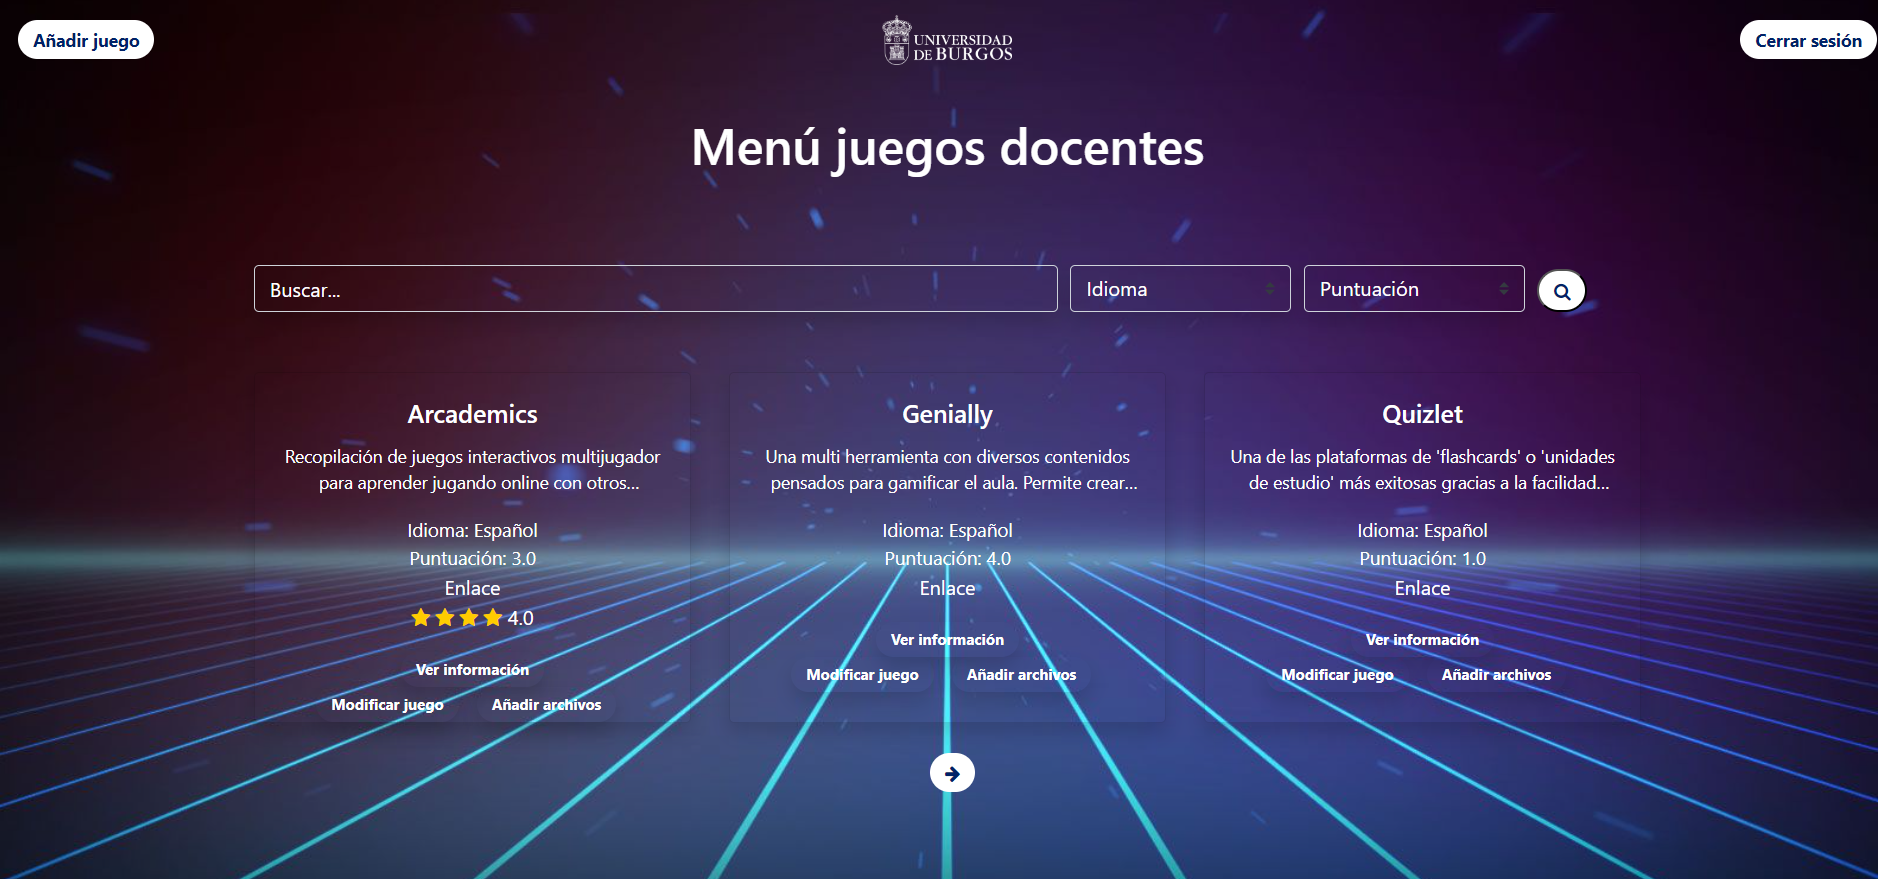
\includegraphics[width=0.8\textwidth]{menu-profesor}
\caption{Interfaz del menú de juegos de profesores.}
\label{fig:menu-profesor}
\end{figure}

Como se puede observar, el resultado final del menu\_juegos\_profesor.html presenta varias diferencias visuales en comparación con el prototipo inicial, al igual que con el menú de juegos de los usuarios. En el resultado final, la visualización de los juegos se presenta en tarjetas, lo cual facilita su visualización y ofrece una apariencia más atractiva. Además, se ha agregado la funcionalidad de realizar búsquedas utilizando tanto la barra de búsqueda como filtros, lo cual permite realizar búsquedas más específicas, al igual que en el menú de los usuarios. También se ha añadido un botón adicional para la subida de archivos a cada juego.

\subsection{Añadir nuevo juego}
La interfaz para añadir un juego nuevo está diseñada exclusivamente para los profesores. En el prototipo, se divide en diferentes secciones donde se debe ingresar información obligatoria sobre el juego que se desea incluir.

\begin{itemize}
    \item Categorización del juego: permite incluir el nombre del juego, su enlace si existe, su disciplina, su naturaleza, el idioma, el precio, las instrucciones del jugador y las notas para el instructor.
    \begin{figure}[htb]
    \centering
    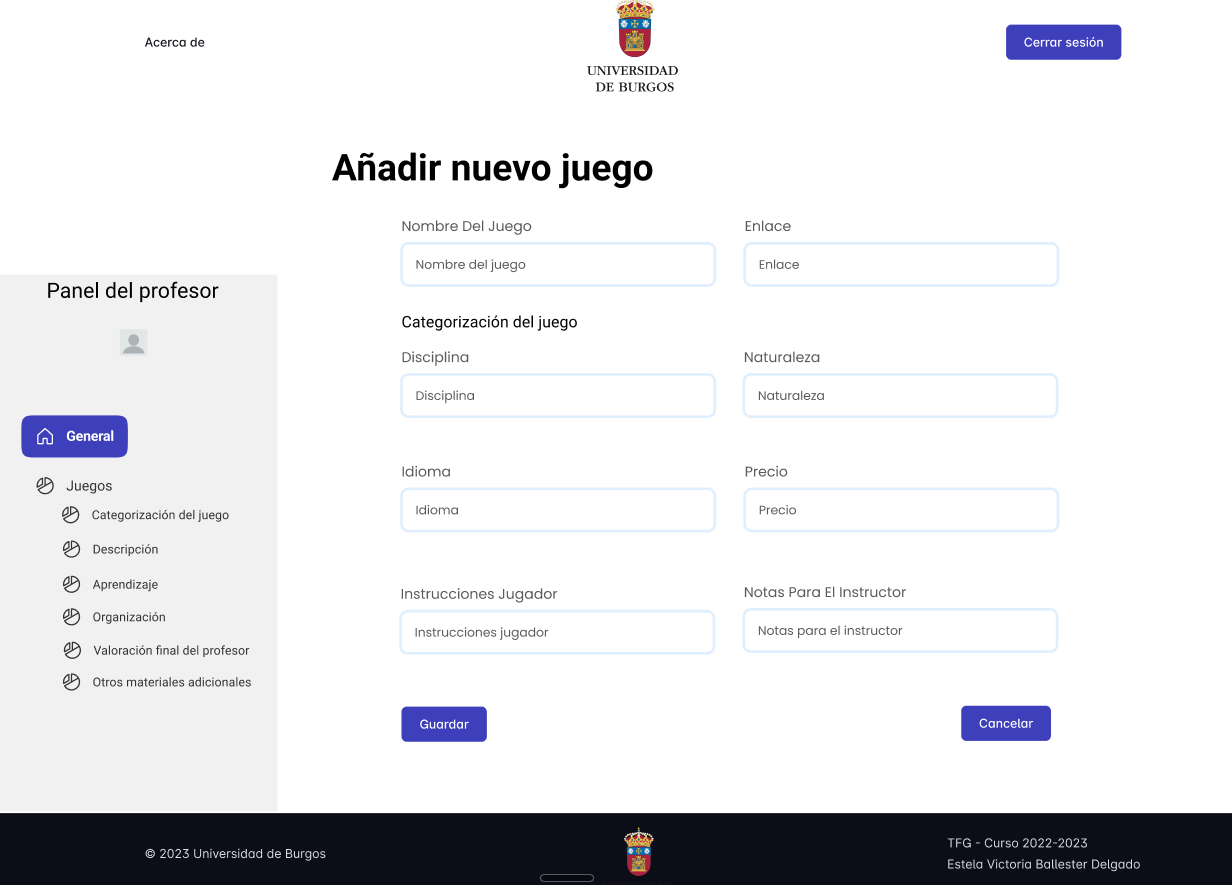
\includegraphics[width=0.7\textwidth]{añadir-juego1-prototipo}
    \caption{Prototipo de añadir la categorización del juego.}
    \label{fig:añadir-juego1-prototipo}
    \end{figure}
    \newpage
    \item Descripción: permite incluir el contexto del juego, los objetivos y el espacio de control.
    \begin{figure}[htb]
    \centering
    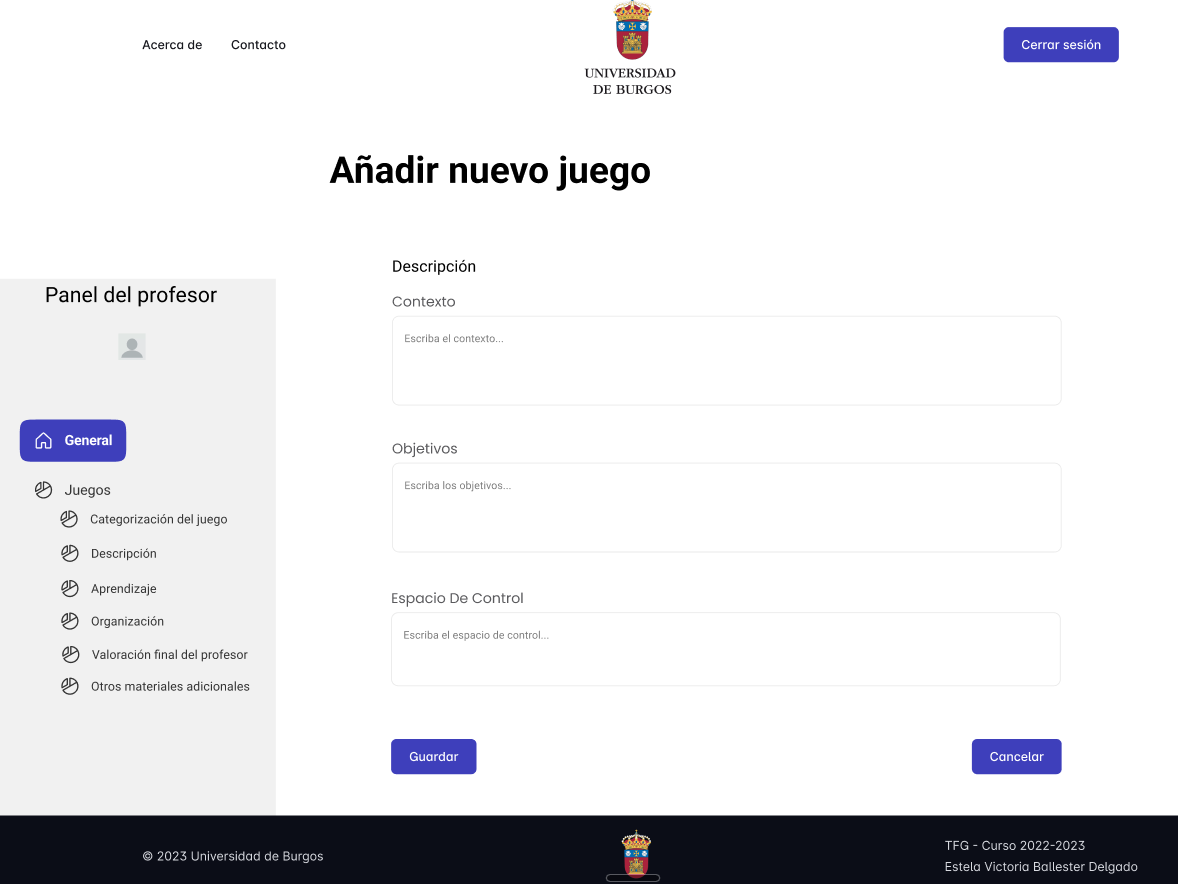
\includegraphics[width=0.7\textwidth]{añadir-juego2-prototipo}
    \caption{Prototipo de añadir la descripción del juego.}
    \label{fig:añadir-juego2-prototipo}
    \end{figure}
 
    \item Aprendizaje: permite incluir los objetivos principales y secundarios.
    \begin{figure}[htb]
    \centering
    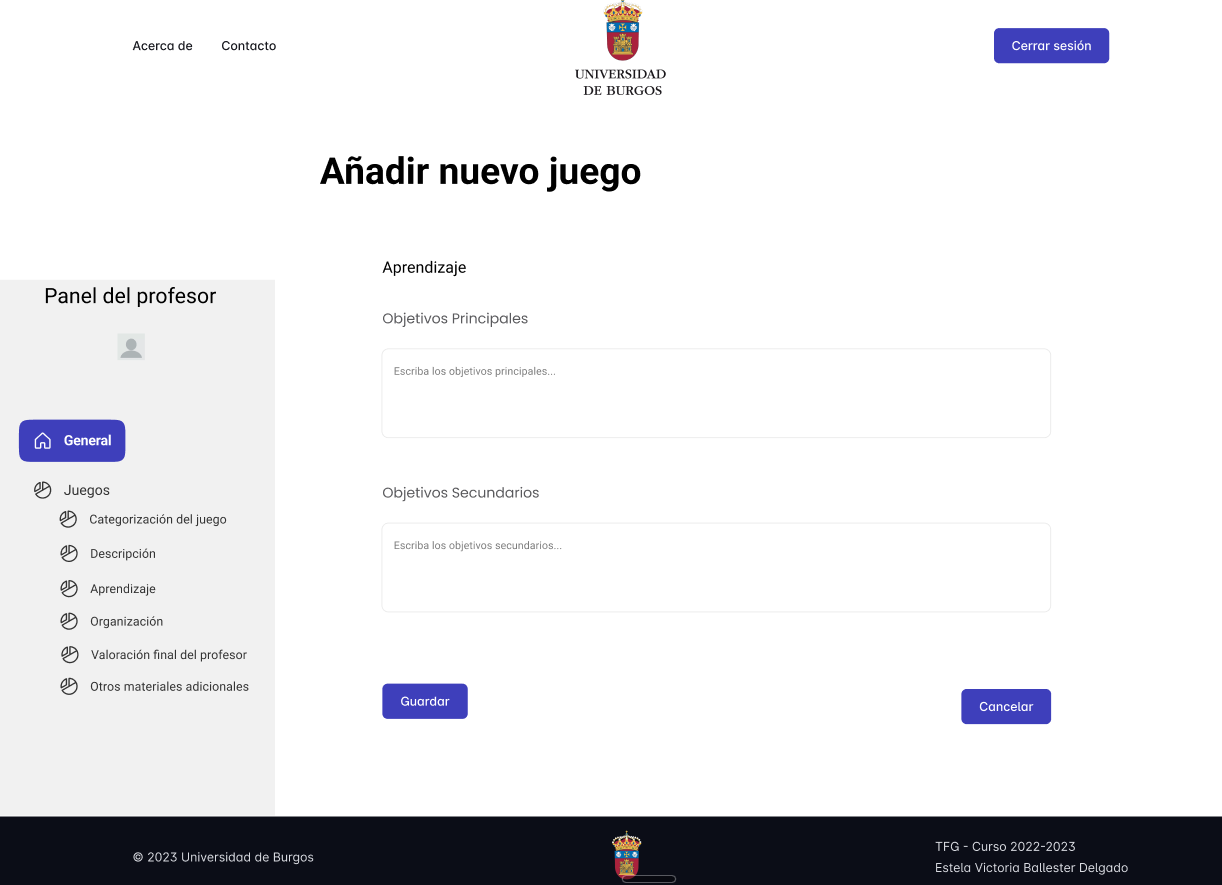
\includegraphics[width=0.7\textwidth]{añadir-juego3-prototipo}
    \caption{Prototipo de añadir el aprendizaje del juego.}
    \label{fig:añadir-juego3-prototipo}
    \end{figure}
    \newpage
    \item Organización: permite incluir la estructura propuesta para las sesiones y los aspectos adicionales a tener en cuenta.
    \begin{figure}[htb]
    \centering
    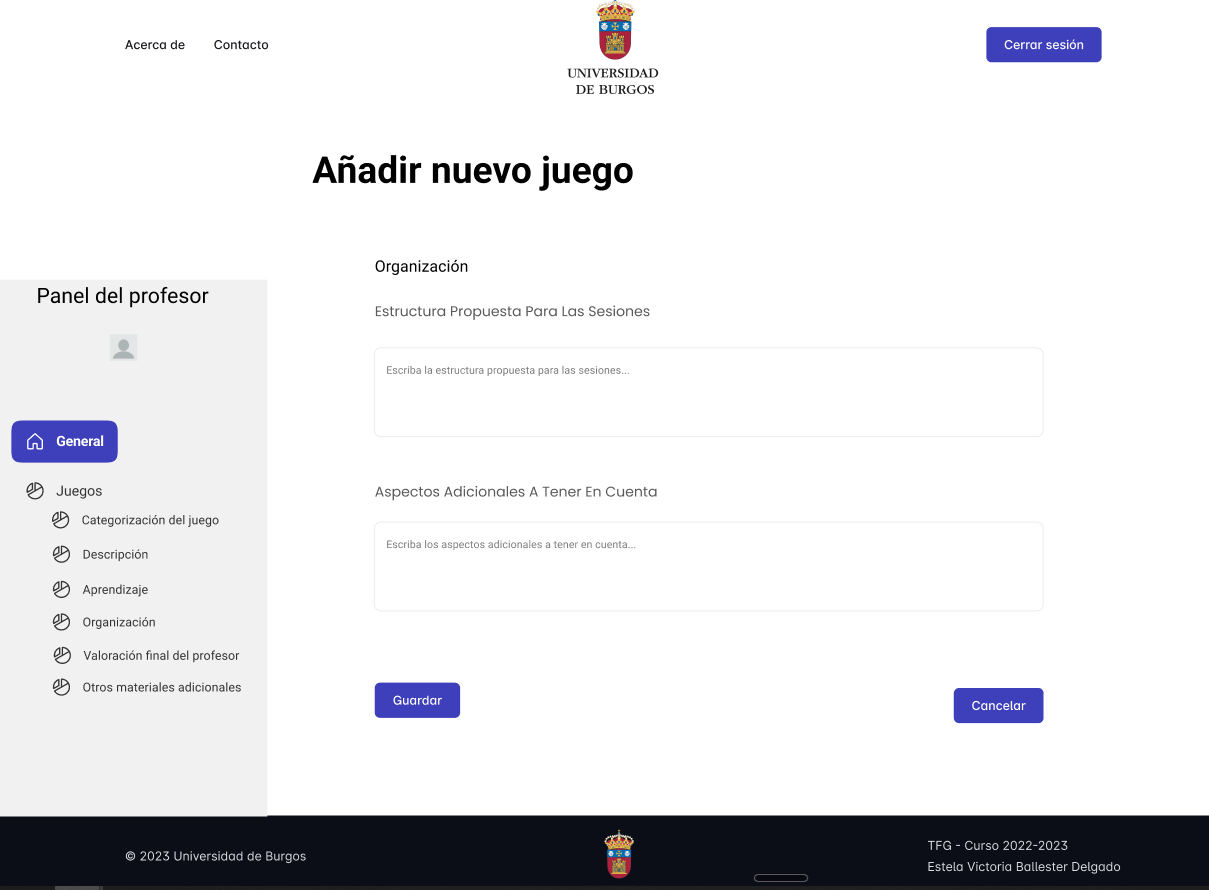
\includegraphics[width=0.6\textwidth]{añadir-juego4-prototipo}
    \caption{Prototipo de añadir la organización del juego.}
    \label{fig:añadir-juego4-prototipo}
    \end{figure}

    \item Valorización final del profesor: permite incluir la valoración del entretenimiento, el aprendizaje, la complejidad para el alumno y la complejidad para nuevos instructores.
    \begin{figure}[htb]
    \centering
    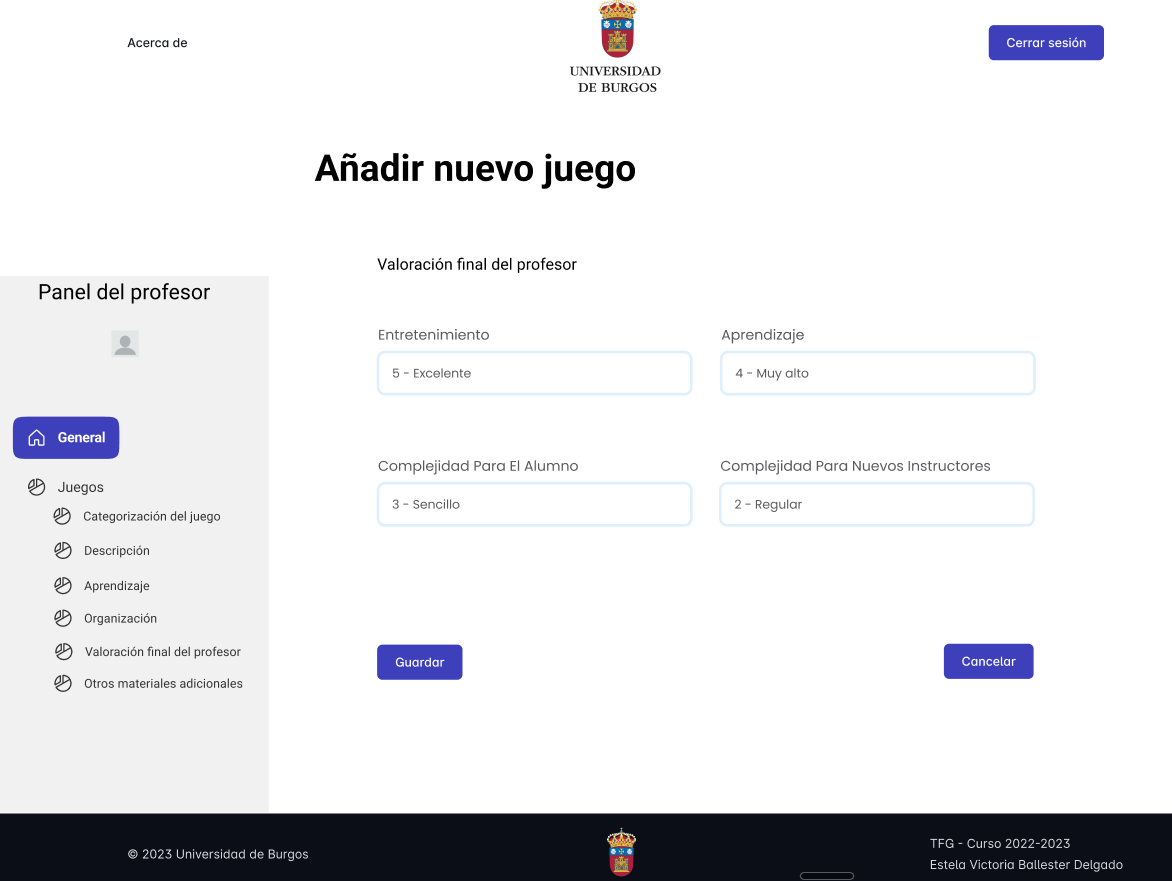
\includegraphics[width=0.7\textwidth]{añadir-juego5-prototipo}
    \caption{Prototipo de añadir la valorización final del profesor del juego.}
    \label{fig:añadir-juego5-prototipo}
    \end{figure}
\end{itemize}
\newpage

Finalmente, el resultado del template añadir\_juego.html quedó de la siguiente manera:

\begin{figure}[htb]
    \centering
    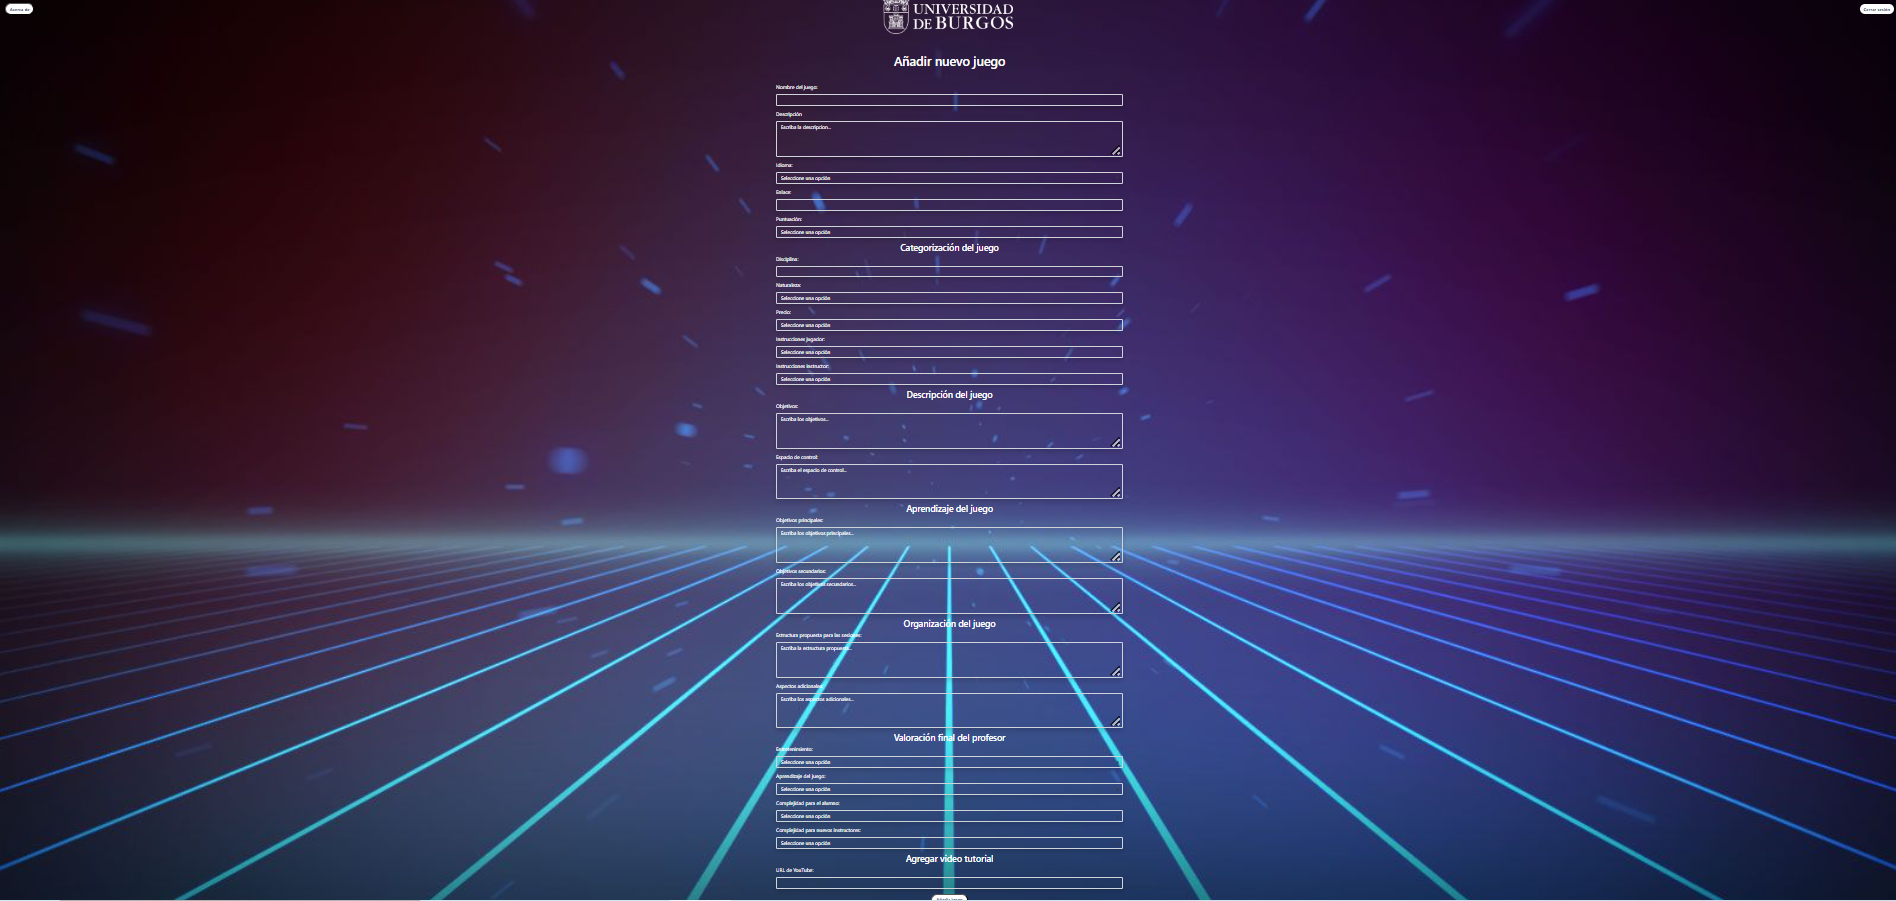
\includegraphics[width=0.8\textwidth]{añadir-juego}
    \caption{Interfaz de añadir juego.}
    \label{fig:añadir-juego}
    \end{figure}

Como se puede observar, el resultado final del template añadir\_juego.html presenta varias diferencias visuales en comparación con el prototipo inicial. En el prototipo, el proceso de añadir un nuevo juego se dividía en diferentes páginas, mientras que en el resultado final se ha unificado todo en una sola página. Además, se ha implementado la opción de añadir un enlace para un vídeo tutorial.

\subsection{Menú de juegos del administrador}
La interfaz del menú de juegos del administrador proporciona diversas funcionalidades. Permite realizar búsquedas personalizadas de los juegos, visualizar información detallada de cada juego, así como acceder al menú de administración.
\newpage

\begin{figure}[htb]
\centering
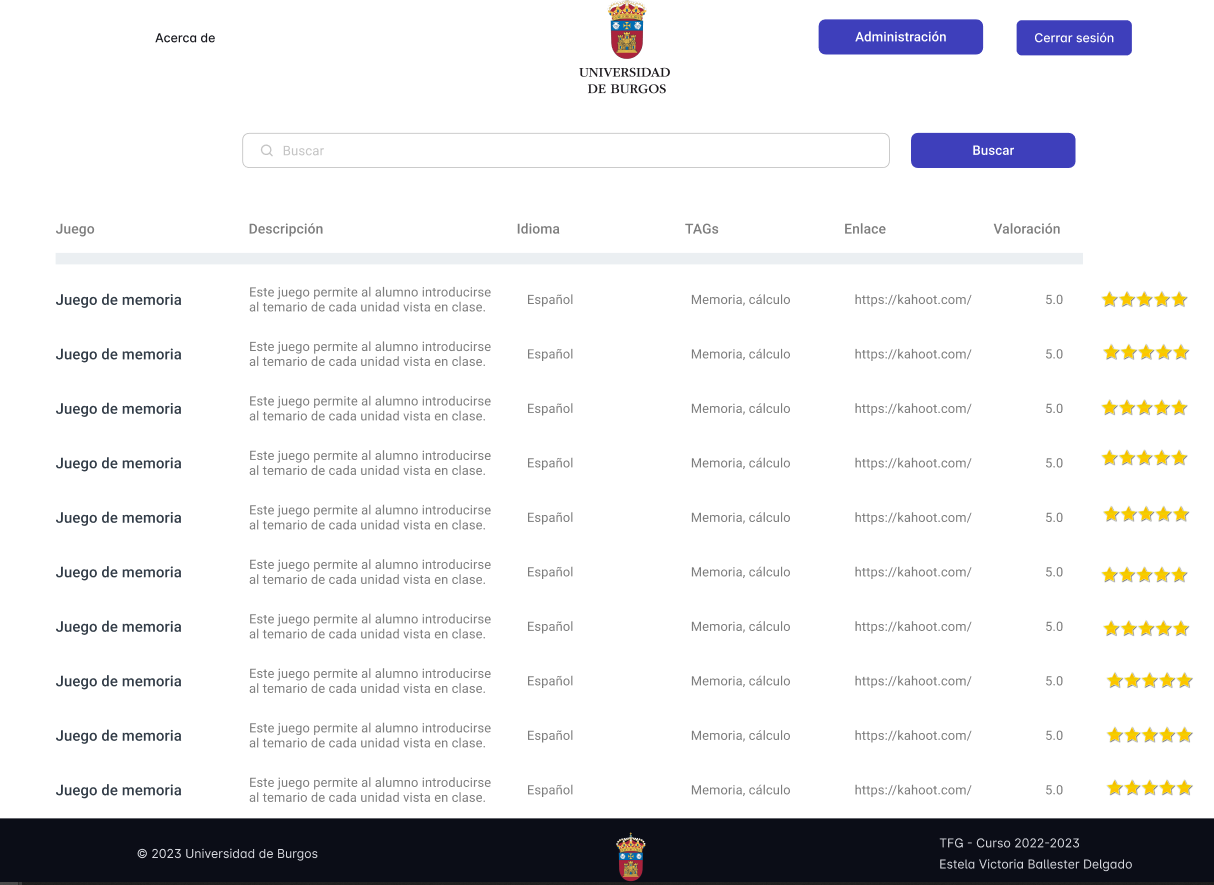
\includegraphics[width=0.7\textwidth]{menu-administrador-prototipo}
\caption{Prototipo del menú de juegos del administrador.}
\label{fig:menu-administrador-prototipo}
\end{figure}

Finalmente, el resultado del template menu\_juegos\_administrador.html quedó de la siguiente manera:

\begin{figure}[htb]
\centering
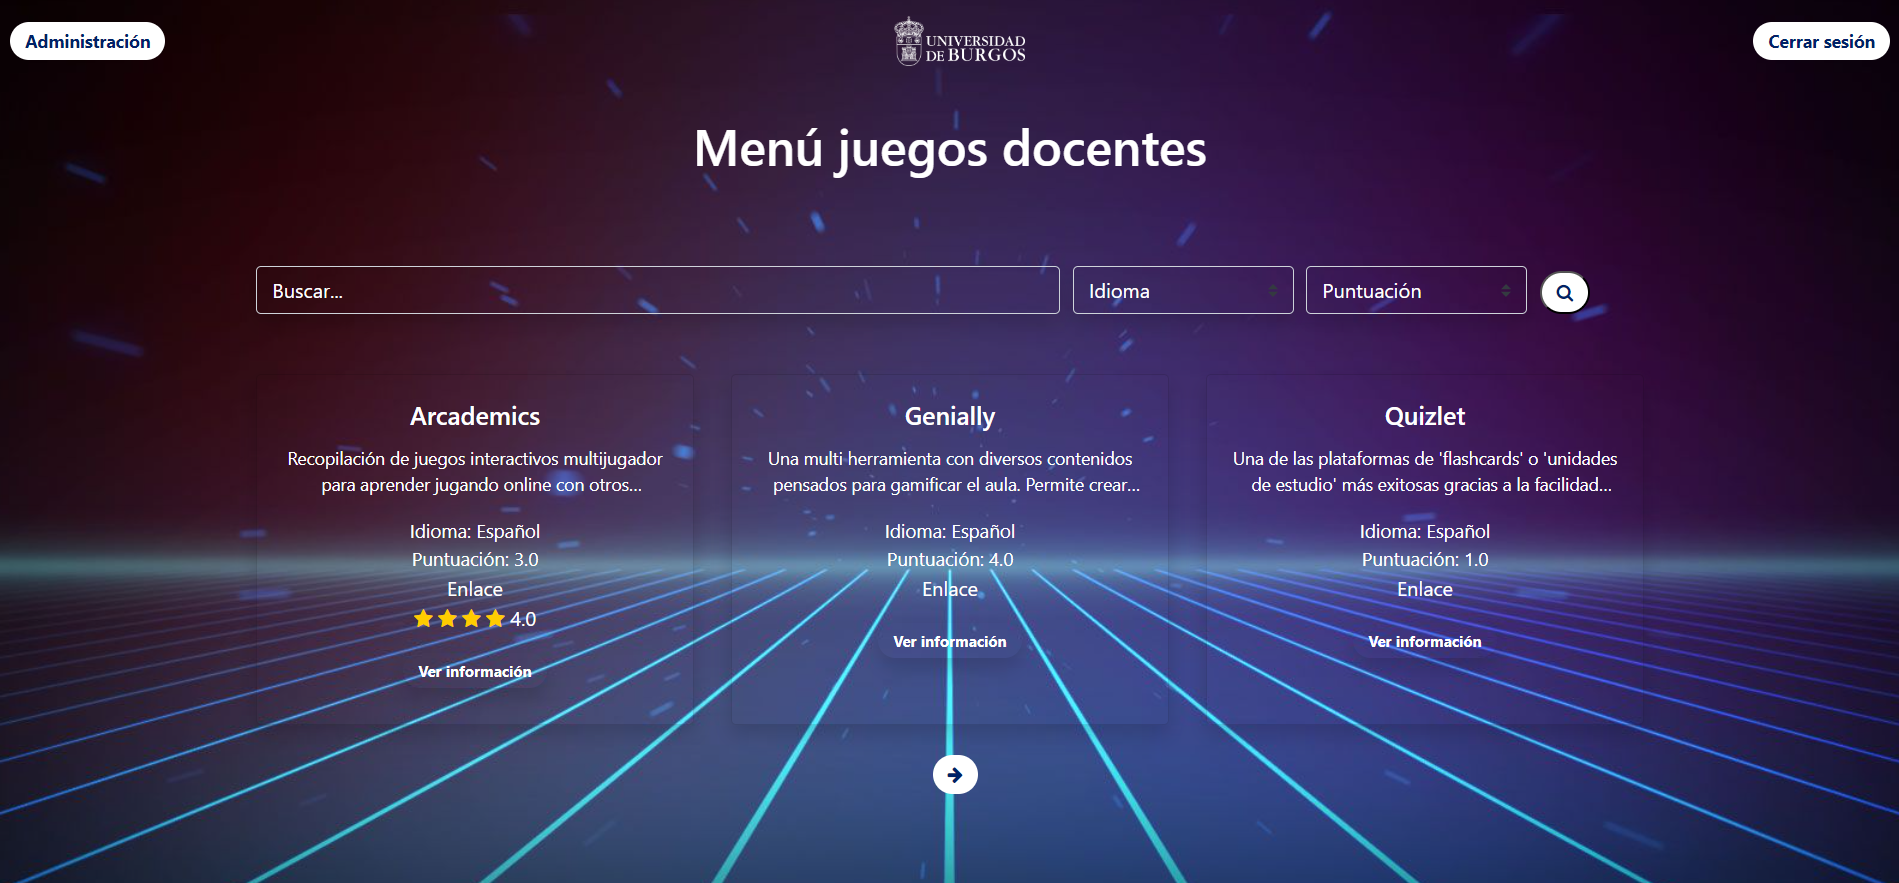
\includegraphics[width=0.8\textwidth]{menu-administrador}
\caption{Interfaz del menú de juegos del administrador.}
\label{fig:menu-administrador}
\end{figure}

Como se puede observar, el resultado final del template menu\_juegos\_administrador.html presenta varias diferencias visuales en comparación con el prototipo inicial, especialmente en lo que respecta a la visualización de los juegos. En el resultado final, se ha implementado la aplicación de filtros, al igual que en los otros menús, lo cual permite una búsqueda más precisa y específica de los juegos disponibles.

\subsection{Administración}
La interfaz de administración permite acceder a las funciones de gestión de juegos, usuarios y solicitudes.

\begin{figure}[htb]
\centering
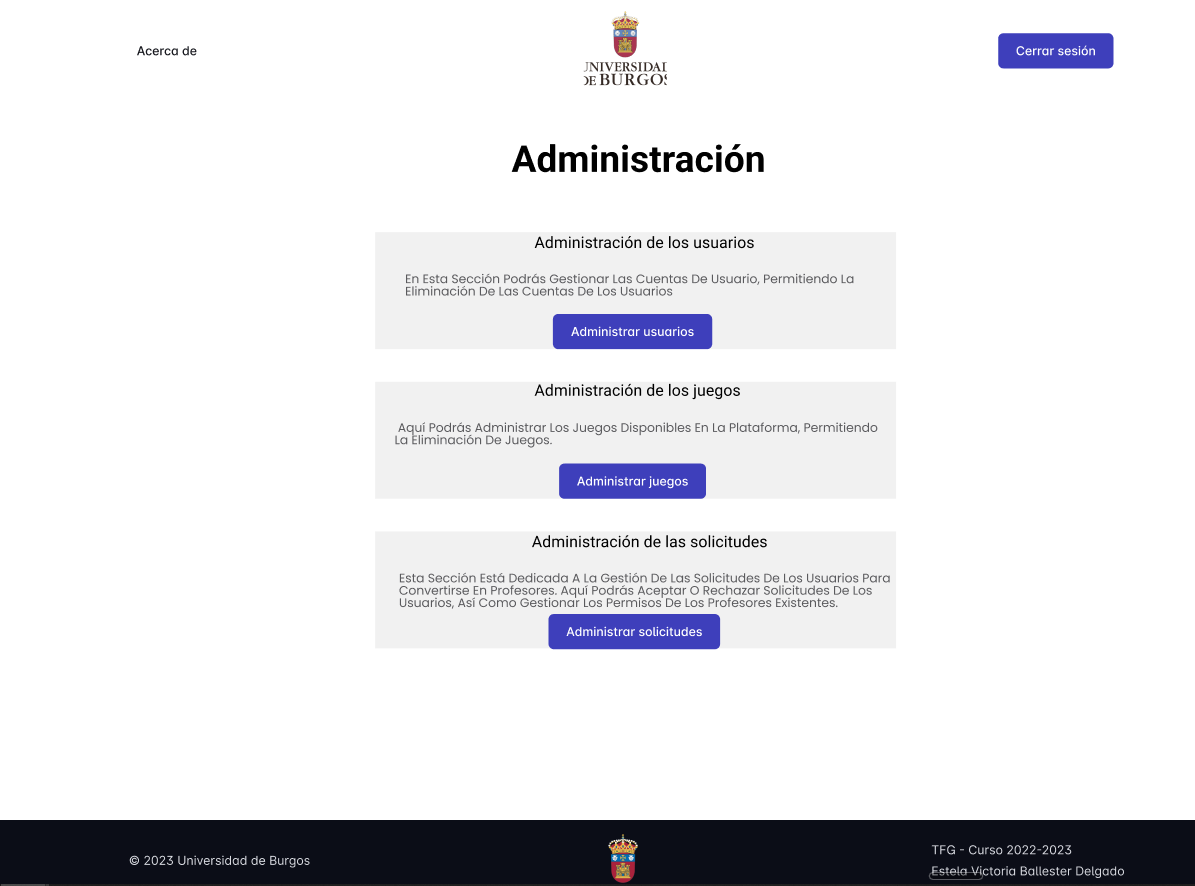
\includegraphics[width=0.7\textwidth]{administracion-prototipo}
\caption{Prototipo de la administración.}
\label{fig:administracion-prototipo}
\end{figure}

Finalmente, el resultado del template administracion.html quedó de la siguiente manera:

\begin{figure}[htb]
\centering
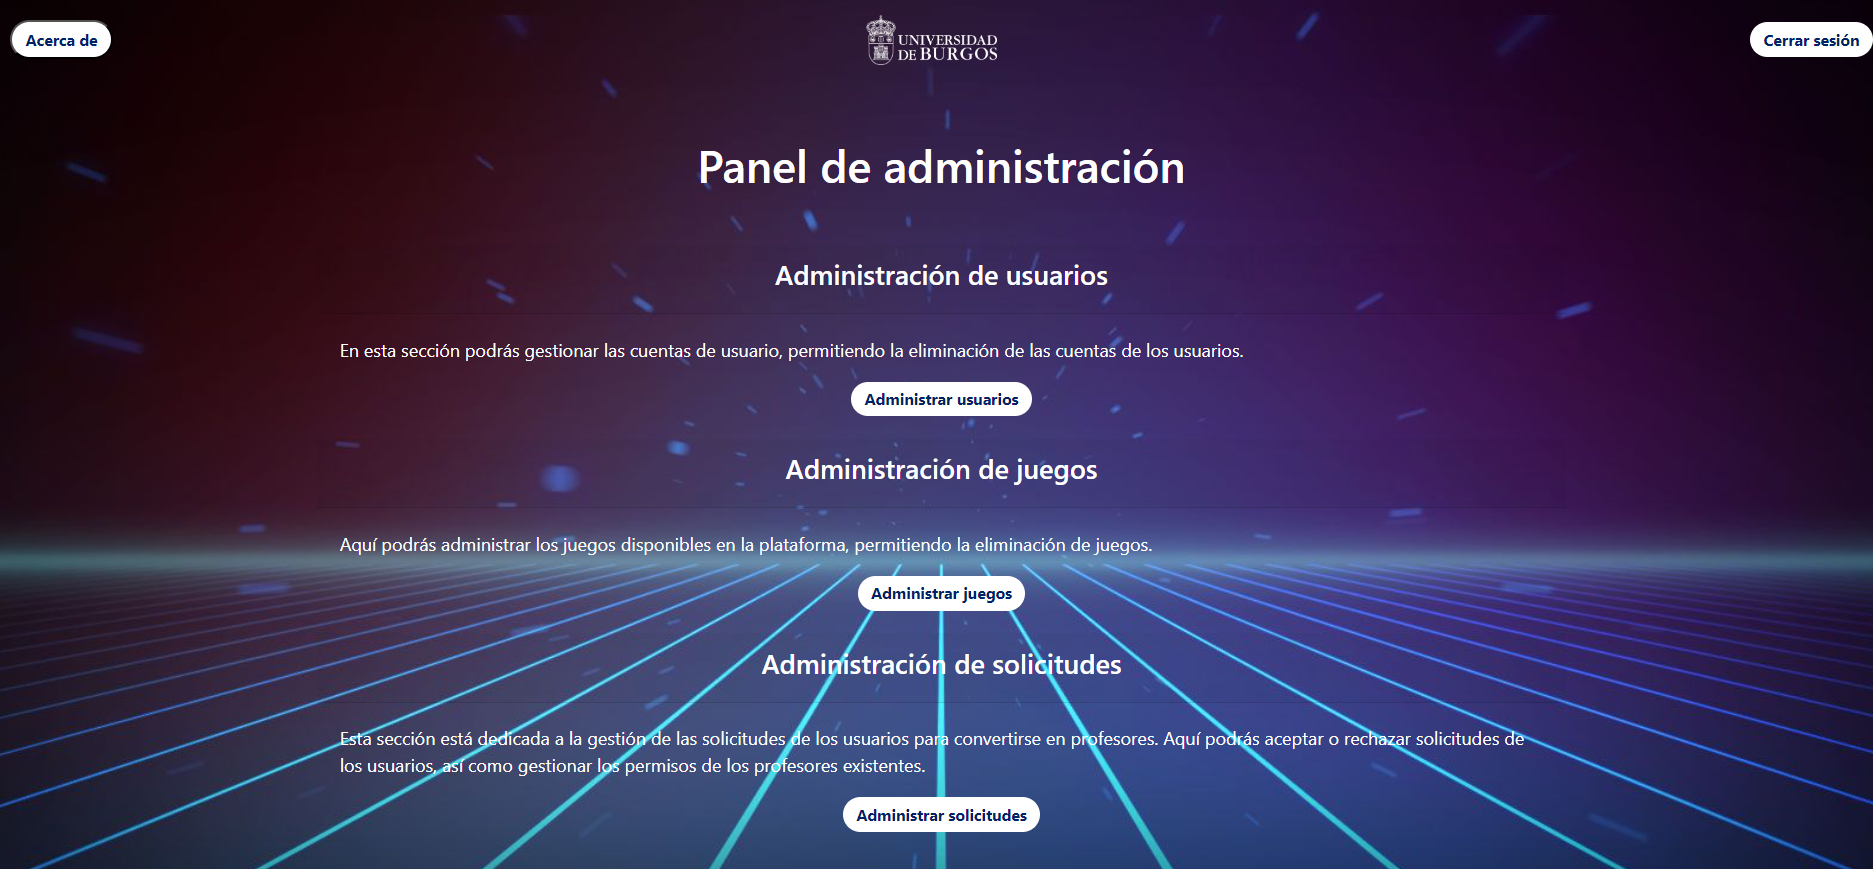
\includegraphics[width=0.8\textwidth]{administracion}
\caption{Interfaz de la administración.}
\label{fig:administracion}
\end{figure}

Como se puede observar, el resultado final del template administracion.html es prácticamente idéntico al prototipo inicial. 

\subsection{Administrar juegos}
La interfaz de los juegos solo es accesible por los administradores. Esta les permite visualizar información general de los juegos y borrarlos en el caso de que sea necesario.

\begin{figure}[htb]
\centering
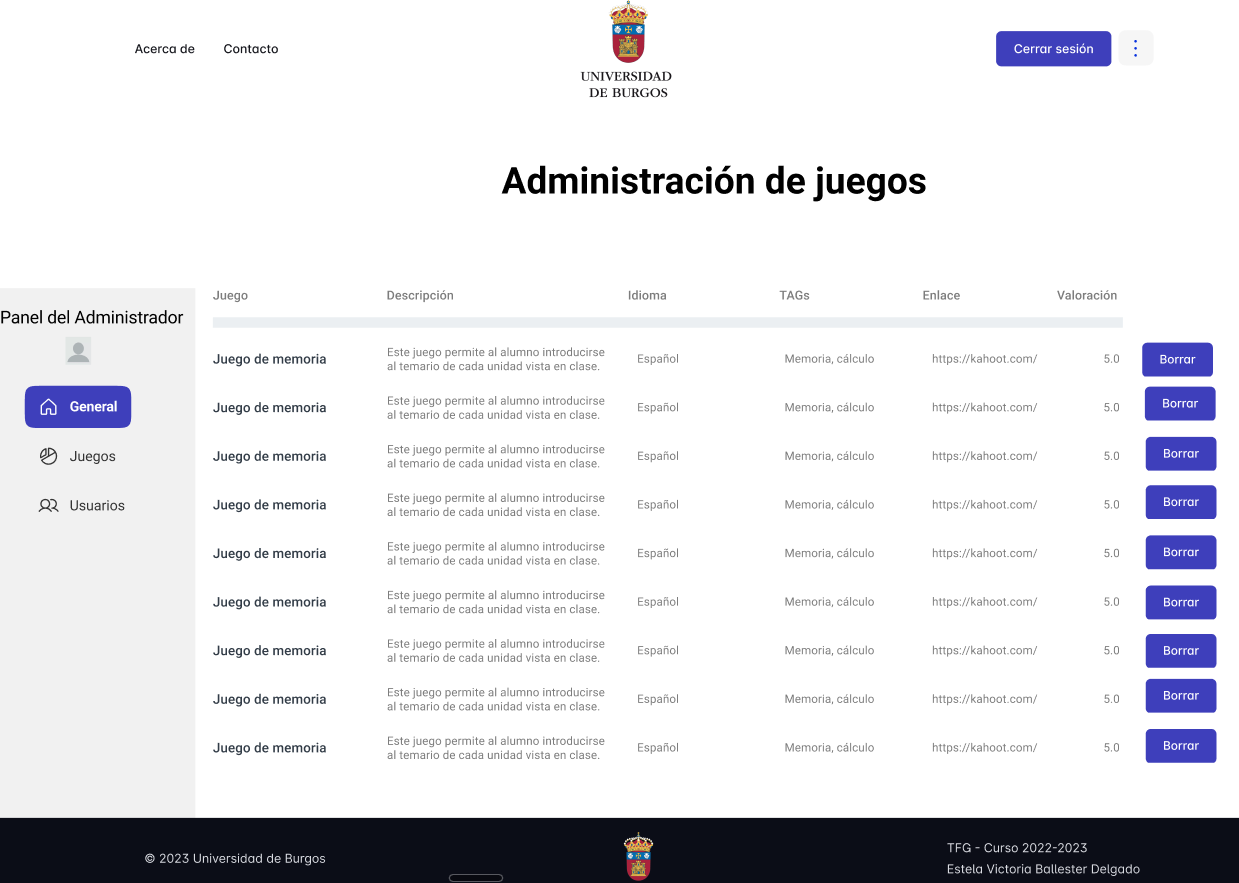
\includegraphics[width=0.7\textwidth]{admin-juegos-prototipo}
\caption{Prototipo de la administración de juegos.}
\label{fig:admin-juegos-prototipo}
\end{figure}

Finalmente, el resultado del template administrar\_juegos.html quedó de la siguiente manera:

\begin{figure}[htb]
\centering
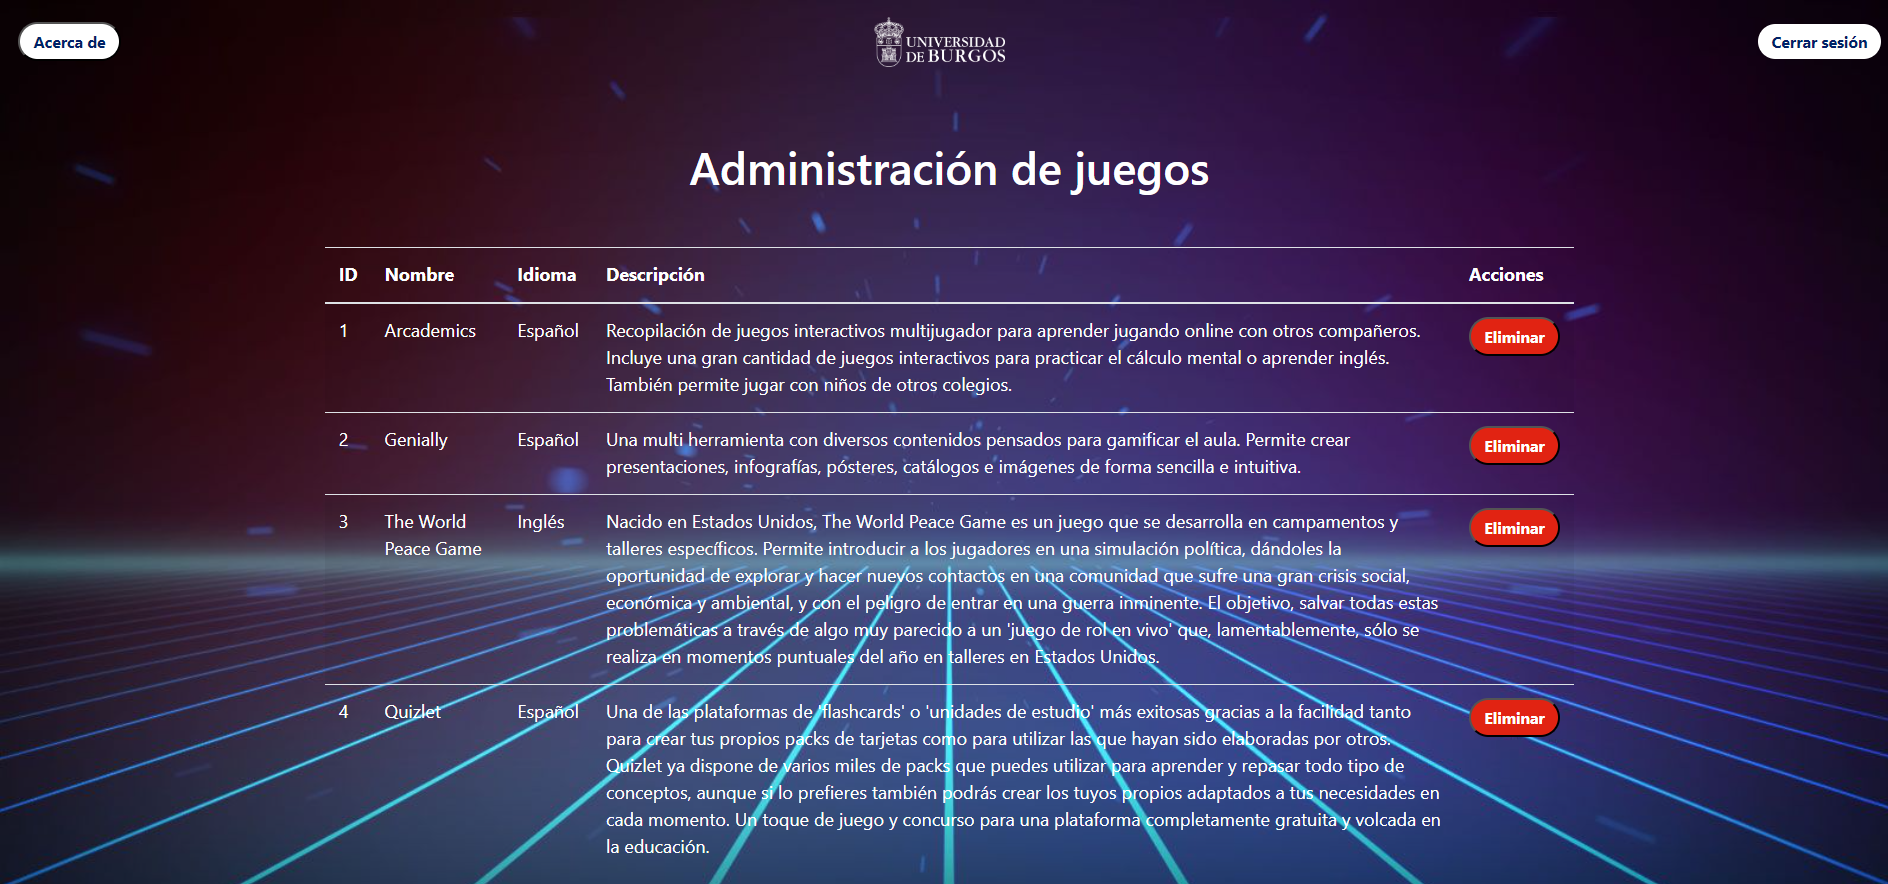
\includegraphics[width=0.8\textwidth]{administracion-juegos}
\caption{Interfaz de la administración de juegos.}
\label{fig:administracion-juegos}
\end{figure}

Como se puede observar, el resultado final del template administrar\_juegos.html es prácticamente idéntico al prototipo inicial. 

\subsection{Administrar usuarios}
La interfaz de gestión de los usuarios solo es accesible por los administradores. Esta les permite visualizar información general de los usuarios y borrarlos en el caso de que sea necesario.
\begin{figure}[htb]
\centering
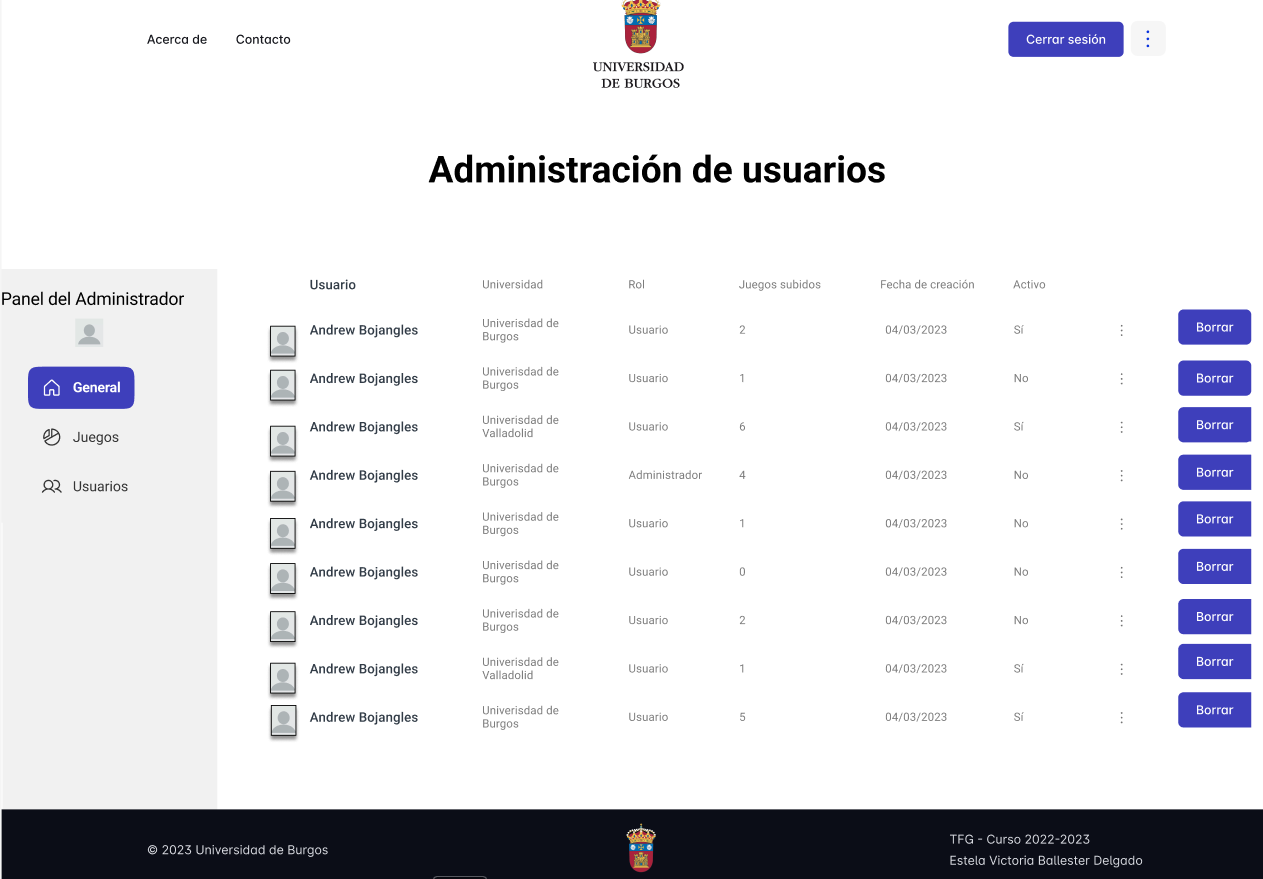
\includegraphics[width=0.7\textwidth]{admin-ususarios-prototipo}
\caption{Prototipo de la administración de los usuarios}
\label{fig:admin-ususarios-prototipo}
\end{figure}

Finalmente, el resultado del template administrar\_usuarios.html quedó de la siguiente manera:

\begin{figure}[htb]
\centering
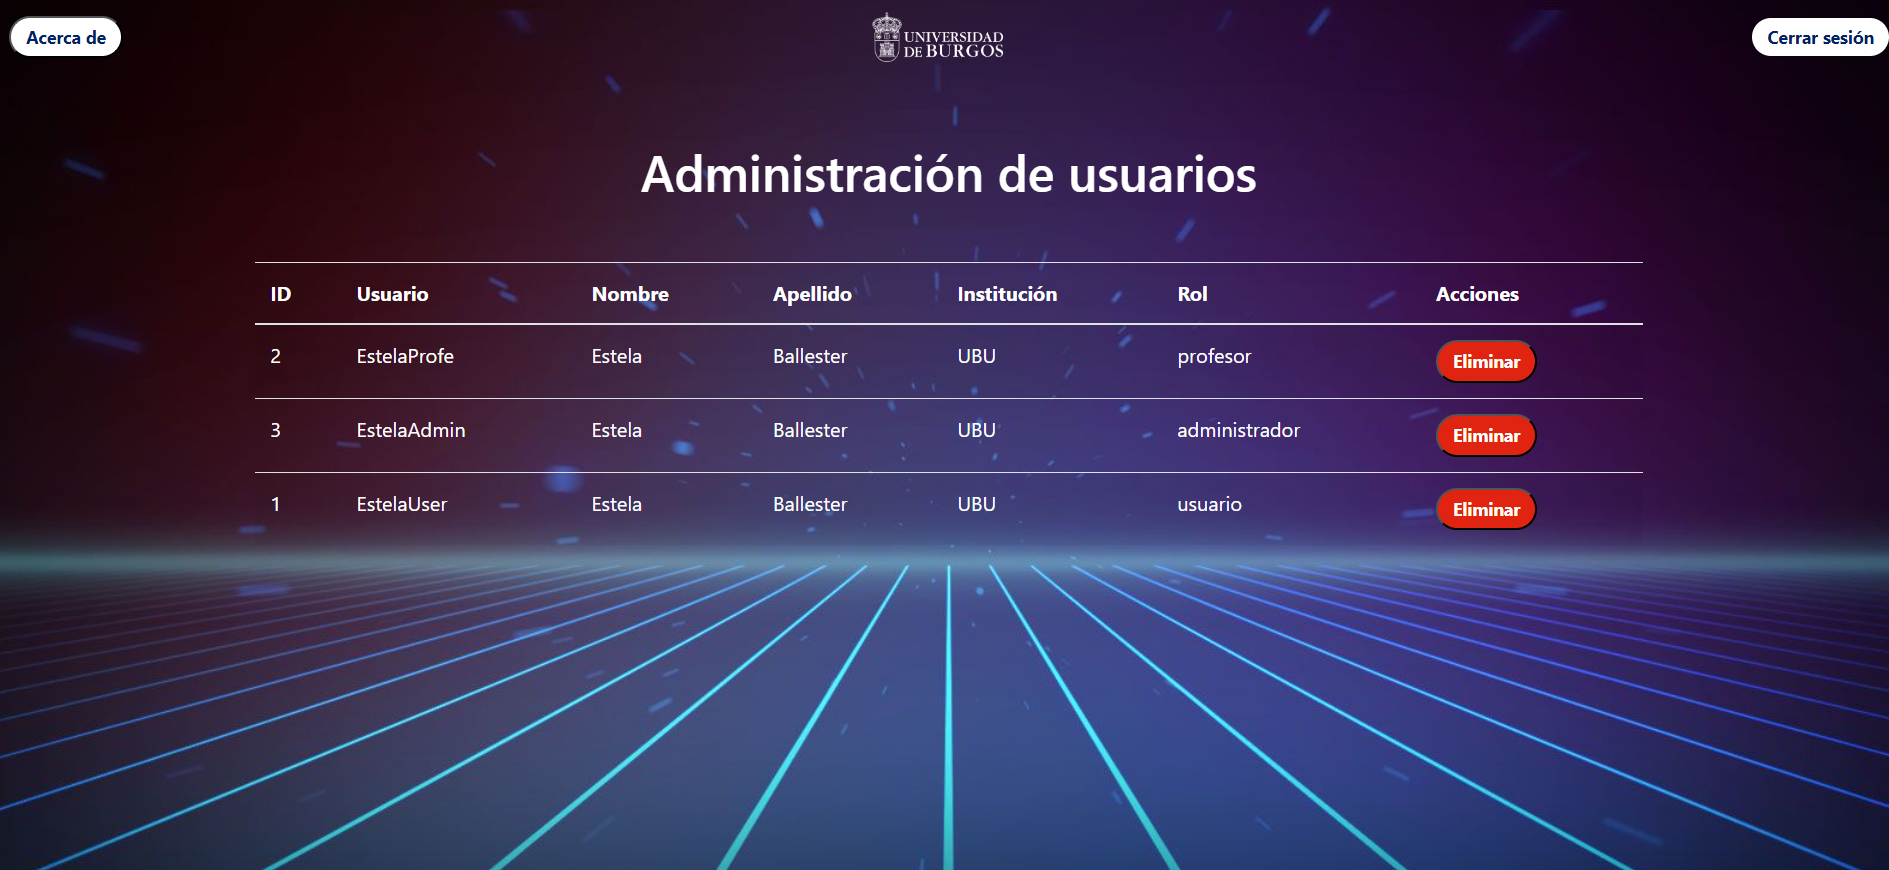
\includegraphics[width=0.8\textwidth]{administracion-usuarios}
\caption{Interfaz de la administración de usuarios.}
\label{fig:administracion-usuarios}
\end{figure}

Como se puede observar, el resultado final del template administrar\_usuarios.html es prácticamente idéntico al prototipo inicial. 

\subsection{Administrar solicitudes}
La interfaz de gestión de las solicitudes solo es accesible por los administradores. Esta les permite visualizar información general de las solicitudes y aprobarlas o rechazarlas.

\begin{figure}[htb]
\centering
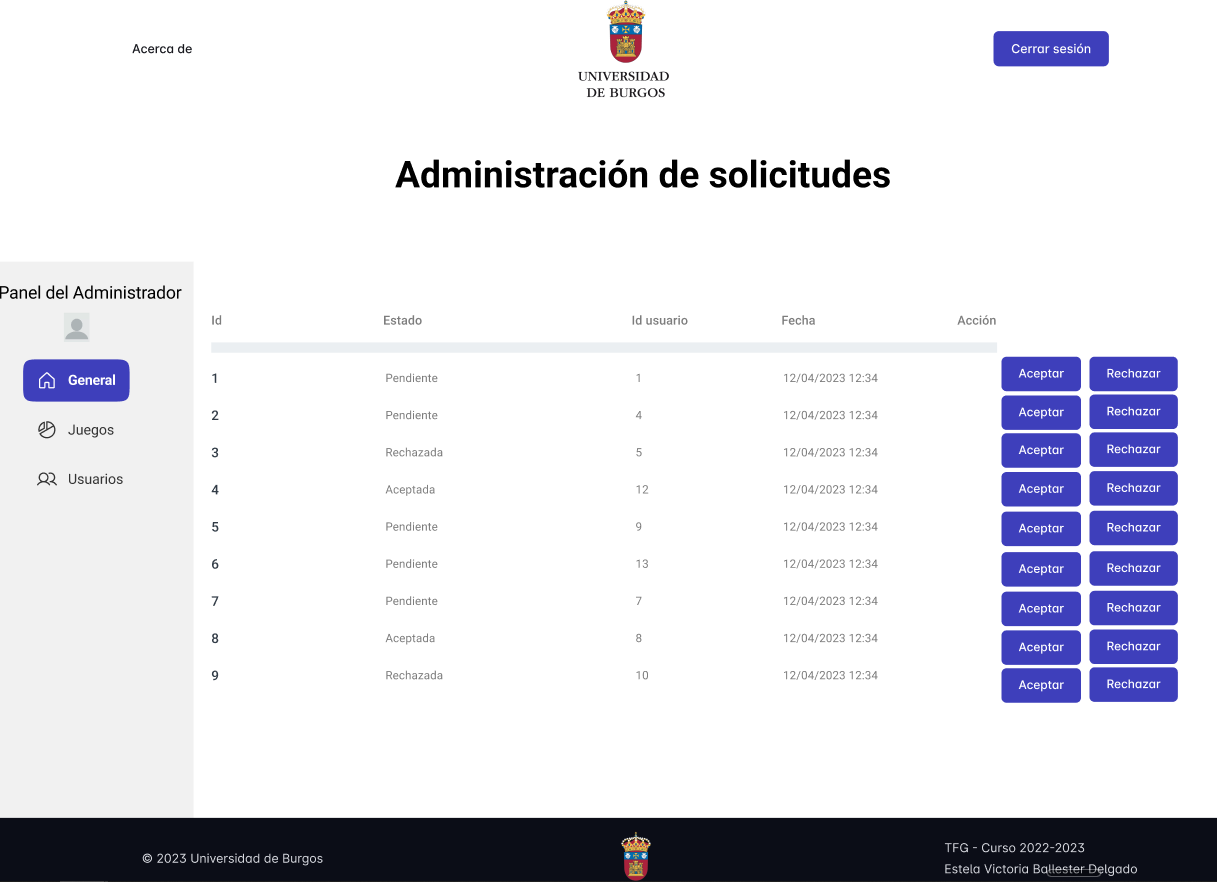
\includegraphics[width=0.7\textwidth]{admin-solicitudes-prototipo}
\caption{Prototipo de la administración de las solicitudes}
\label{fig:admin-solicitudes-prototipo}
\end{figure}
Finalmente, el resultado del template administrar\_solicitudes.html quedó de la siguiente manera:

\begin{figure}[htb]
\centering
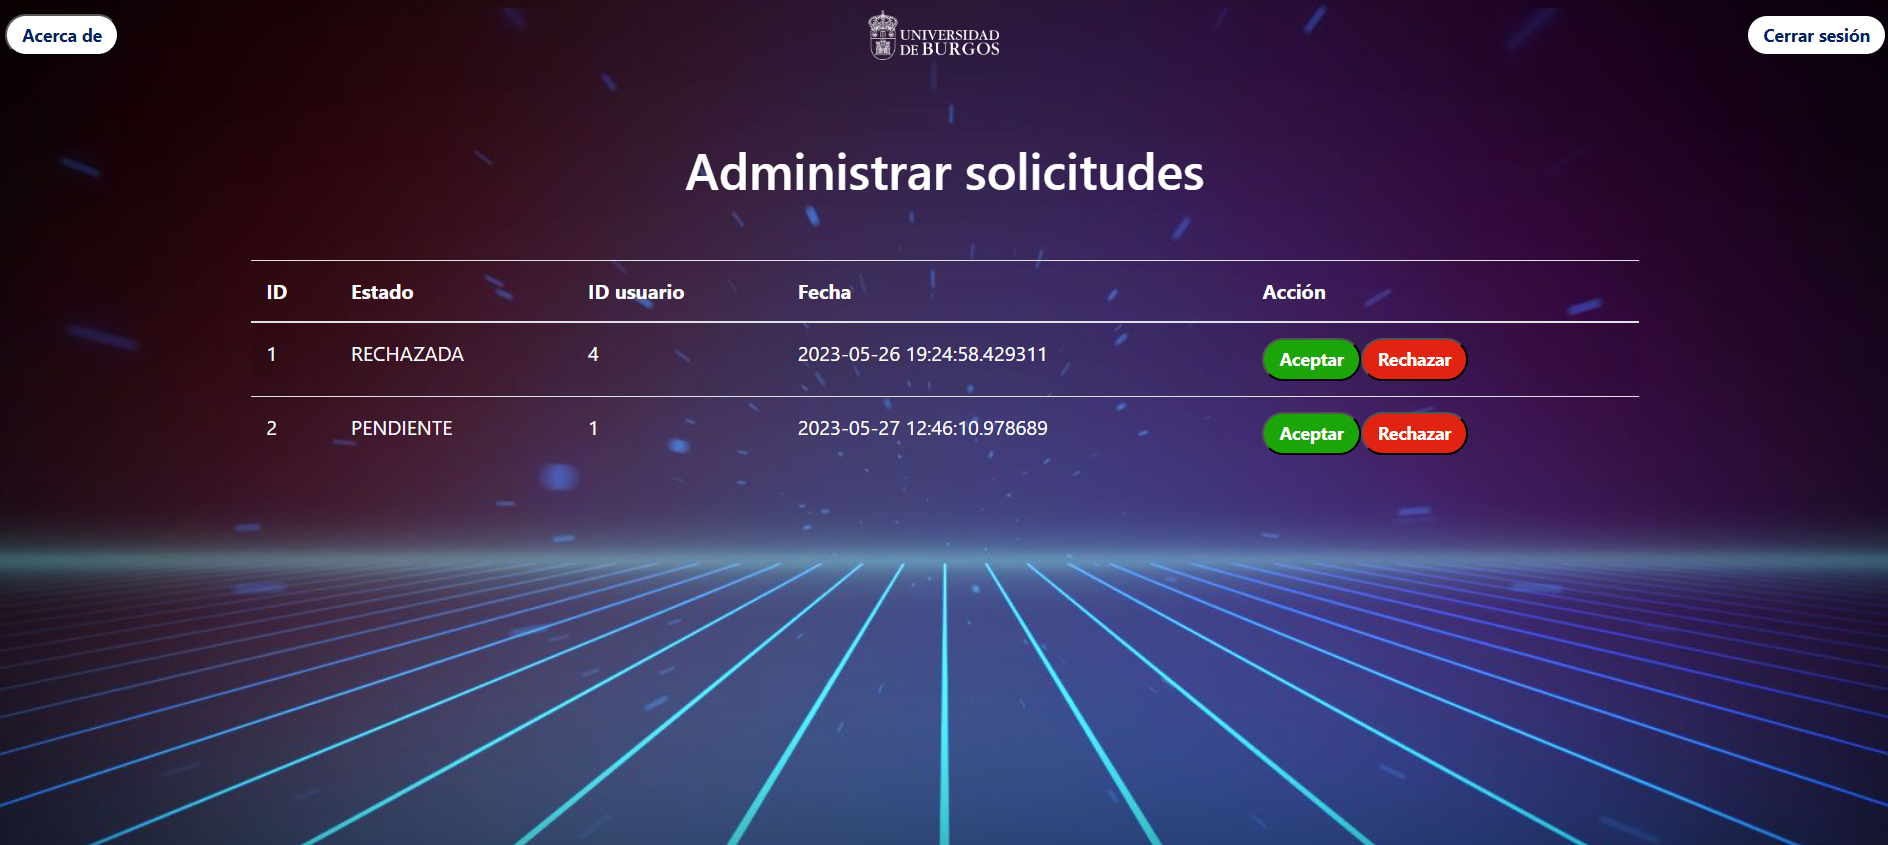
\includegraphics[width=0.8\textwidth]{administracion-solicitudes}
\caption{Interfaz de la administración de solicitudes.}
\label{fig:administracion-solicitudes}
\end{figure}

Como se puede observar, el resultado final del template administrar\_solicitudes.html es prácticamente idéntico al prototipo inicial. 

\subsection{Acerca de}
La interfaz de acerca está disponible para todos los usuarios, independientemente de su rol. En esta página se muestra información general sobre la aplicación.

\begin{figure}[htb]
\centering
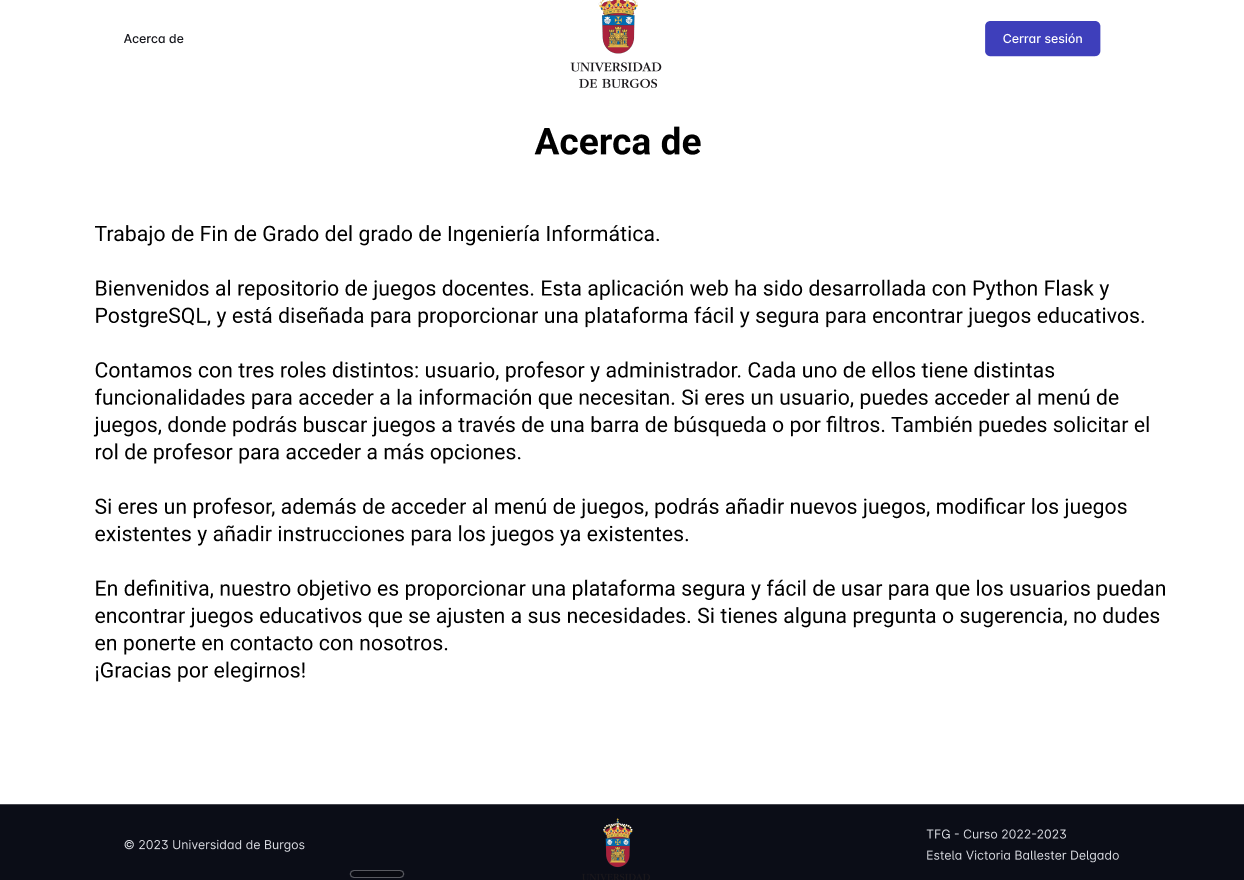
\includegraphics[width=0.7\textwidth]{acerca-prototipo}
\caption{Prototipo de acerca de.}
\label{fig:acerca-prototipo}
\end{figure}
Finalmente, el resultado del template acerca\_de.html quedó de la siguiente manera:

\begin{figure}[htb]
\centering
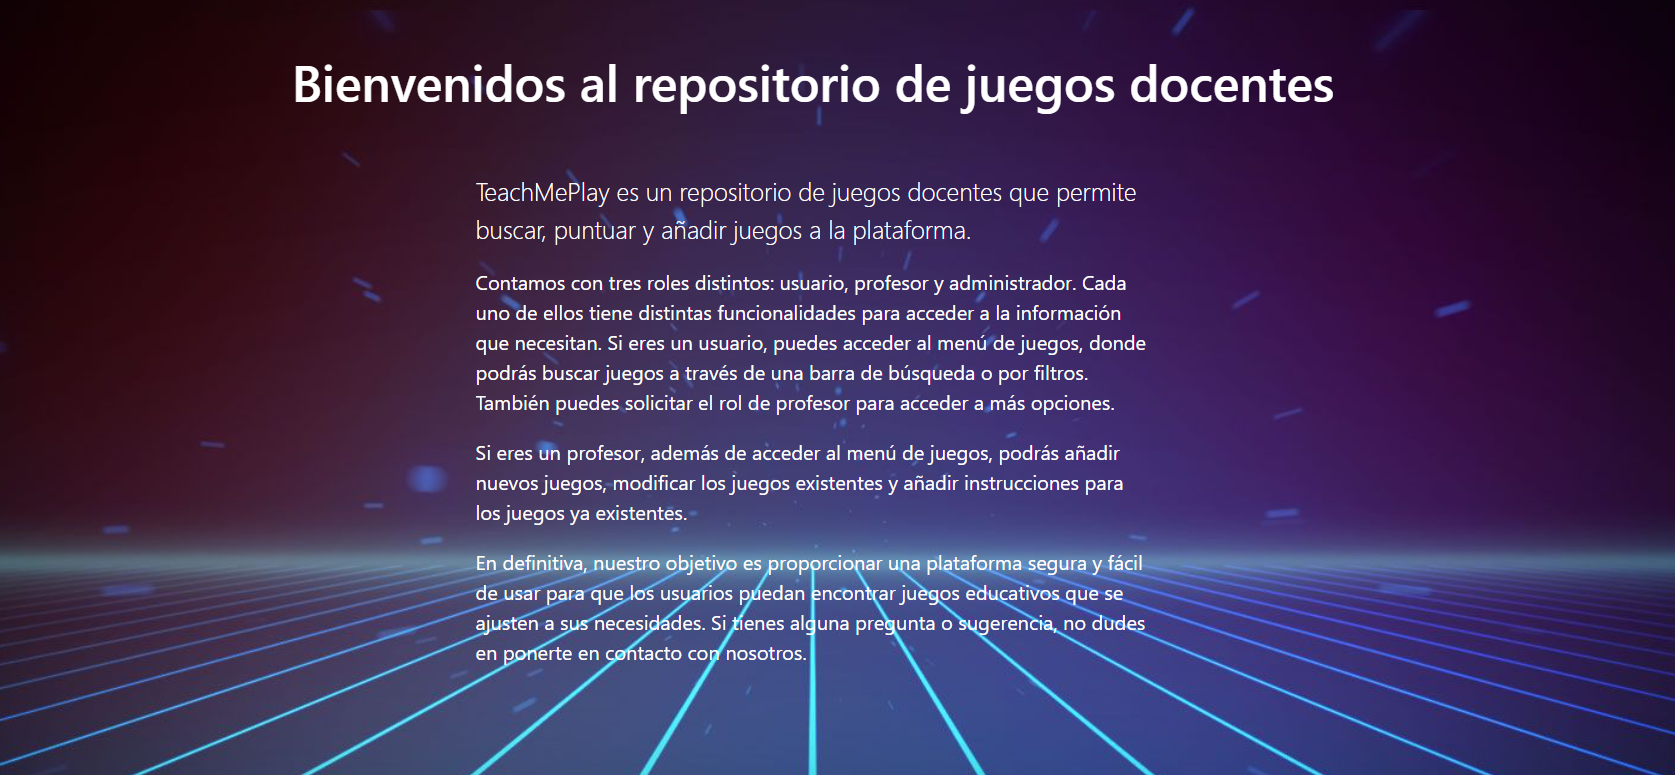
\includegraphics[width=0.8\textwidth]{acerca}
\caption{Interfaz de acerca de.}
\label{fig:acerca}
\end{figure}

Como se puede observar, el resultado final del template acerca\_de.html es prácticamente idéntico al prototipo inicial. 

\subsection{Modificar juego}
La interfaz de modificar un juego permite al profesor modificar la información de cada juego.
\begin{figure}[htb]
\centering
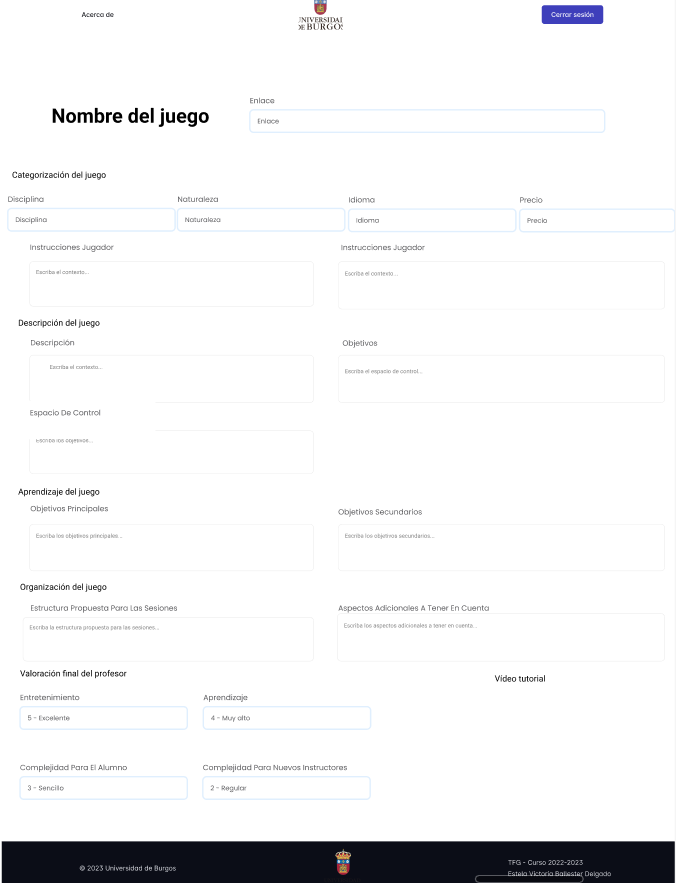
\includegraphics[width=0.7\textwidth]{modificar-juego-prototipo}
\caption{Prototipo de la modificación de juegos.}
\label{fig:modificar-juego-prototipo}
\end{figure}

Finalmente, el resultado del template modificar\_juego.html quedó de la siguiente manera:
\newpage
\begin{figure}[htb]
\centering

\includegraphics[width=0.8\textwidth]{modificar-juego}
\caption{Interfaz de la modificación de juegos.}
\label{fig:modificar-juego}
\end{figure}

Como se puede observar, el resultado final del template modificar\_juego.html es prácticamente idéntico al prototipo inicial. 

\subsection{Visualizar juego}
La interfaz de visualizar un juego permite los usuarios ver la información específica de cada juego.
\newpage
\begin{figure}[htb]
\centering
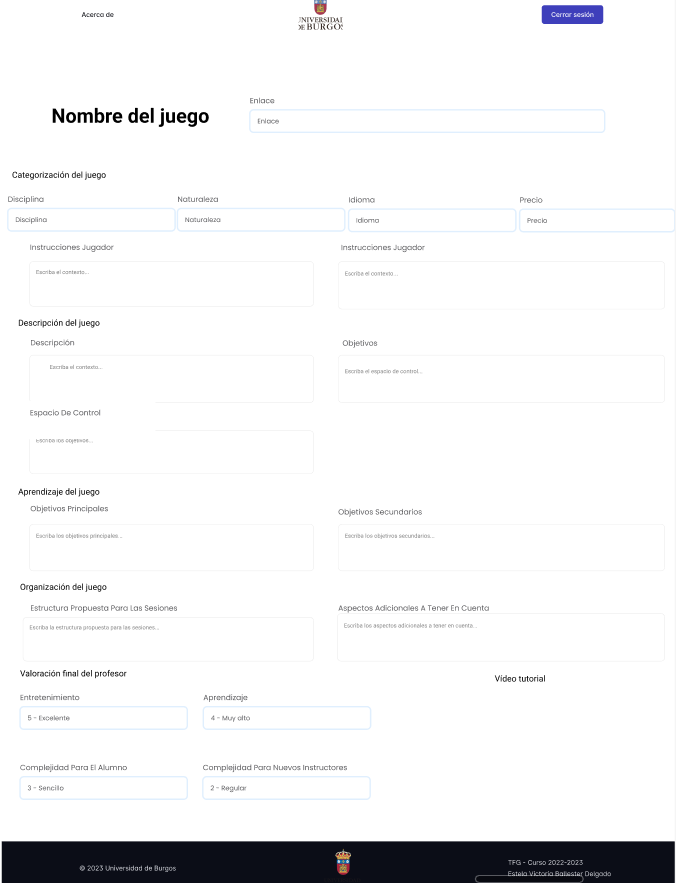
\includegraphics[width=0.7\textwidth]{visualizar-juego-prototipo}
\caption{Prototipo de la visualización de juegos.}
\label{fig:visualizar-juego-prototipo}
\end{figure}
Finalmente, el resultado del template visualizar\_juego.html quedó de la siguiente manera:
\newpage
\begin{figure}[htb]
\centering
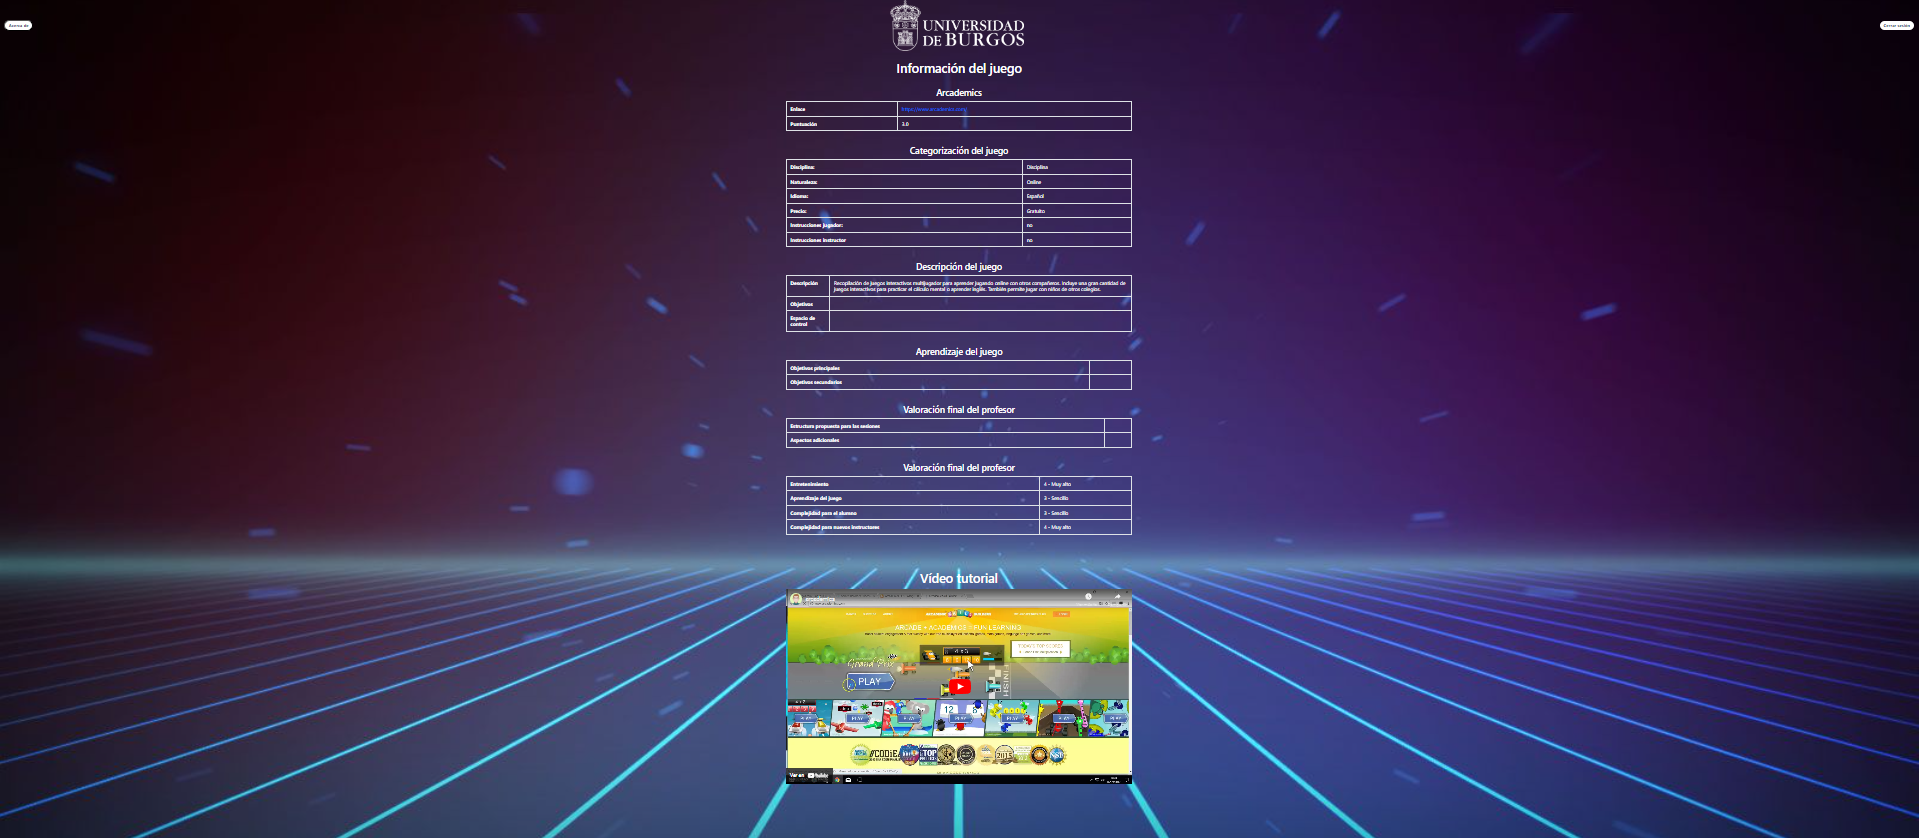
\includegraphics[width=0.8\textwidth]{visualizar-juego}
\caption{Interfaz de la visualización de juegos.}
\label{fig:visualizar-juego}
\end{figure}

Como se puede observar, el resultado final del template visualizar\_juego.html es prácticamente idéntico al prototipo inicial. 

Al tratarse de una aplicación responsive, está disponible para ser utilizada en otros dispositivos. A continuación, se muestra cómo se visualizan las interfaces en un dispositivo móvil.
\begin{figure}[htb]
\centering
\includegraphics[width=0.8\textwidth]{interfaces-movil}
\caption{Interfaces desde dispositivo móvil.}
\label{fig:interfaces-movil}
\end{figure}